%%%%%%%%%%%%%%%%%%%%%%%%%%%%%%%%%%%%%%%%%
% OIST Doctoral Thesis - Final bound version
% LaTeX Template
% Version 0.2 (2016/04/06)
%
% This version is the final binding version which will be published.
%
% Original author:
% Jeremie Gillet
%
%%%%%%%%%%%%%%%%%%%%%%%%%%%%%%%%%%%%%%%%%

%----------------------------------------------------------------------------------------
%	PACKAGES AND OTHER DOCUMENT CONFIGURATIONS
%----------------------------------------------------------------------------------------

\documentclass[12pt, twoside]{book} % 12 pt font, two-sided book style
\usepackage[a4paper, includehead, headheight=0.6cm, inner=3cm ,outer=2.5cm, top=2.5 cm, bottom=2.5cm]{geometry}  % Changing size of document
\usepackage[english]{babel} % The document is in English
\usepackage[utf8]{inputenc} % UTF8 encoding
\usepackage[T1]{fontenc} % Font encoding
\usepackage{float}
\usepackage{subfigure}
\usepackage{longtable}
\usepackage{listings}
\usepackage{url}
\usepackage{graphicx} % For including images
\graphicspath{{./Images/}} % Specifies the directory where pictures are stored

\usepackage{longtable} % tables that can span several pages
\usepackage[bf]{caption} % caption: FIG in bold
\usepackage{fancyhdr} % For the headers
\usepackage{setspace} % For double spacing
\usepackage[table,xcdraw]{xcolor}
\usepackage[figuresright]{rotating}
\newcommand{\numberedchapter}{ % Preparation for numbered chapters
	\cleardoublepage % To make sure the previous headers are passed
	\fancyhead[RE]{{\bfseries \leftmark}}% Headers for left pages
	\fancyhead[LO]{{\bfseries \rightmark}}}% Headers for right pages
\newcommand{\unnumberedchapter}[1]{ % Preparation for unnumbered chapters
	\cleardoublepage % To make sure the previous headers are passed
	\phantomsection % To make sure the table of content links to the right page
	\addcontentsline{toc}{chapter}{#1} % Also adds the chapter name to the Contents
	\fancyhead[RE]{{\bfseries #1}} % Headers for left pages
	\fancyhead[LO]{}}%Headers for right pages

\usepackage{emptypage} % No headers on an empty page

\usepackage{eso-pic} % For the background picture on the title page
\newcommand\BackgroundPic{%
\put(-250,-160){%
\parbox[b][\paperheight]{\paperwidth}{%
\vfill
\centering
\includegraphics[width=\paperwidth]{symbol.jpg}%
\vfill
}}}

\usepackage{hyperref} % Adds clickable links at references

%----------------------------------------------------------------------------------------
%	ADD YOUR CUSTOM VALUES, COMMANDS AND PACKAGES
%----------------------------------------------------------------------------------------

% Open Preamble/mydefinitions.tex and enter some values (name, thesis title...) 
% and include your own custom LaTeX functions and packages

%----------------------------------------------------------------------------------------
%	VALUES FOR THE THESIS
%----------------------------------------------------------------------------------------

\newcommand{\name}{Wenbo Wu} % Author name
\newcommand{\thesistitle}{Data Center Networking} % Title of the thesis
\newcommand{\submissiondate}{April, 2022} % Submission date "Month, year"
\newcommand{\Supervisor}{Shuangyi Yan} % Supervisor name
%\newcommand{\cosupervisor}{C.~O'Supervisor} % Co-Supervisor name, comment this line if there is none


%----------------------------------------------------------------------------------------
%	BIBLIOGRAPHY STYLE (pick the style you want)
%----------------------------------------------------------------------------------------

\usepackage[square, numbers, sort&compress]{natbib} % for bibliography - Square brackets, citing references with numbers, citations sorted by appearance in the text and compressed (as in [4-7])
%\usepackage[longnamesfirst,round]{natbib} % Natural Sciences bibliography

\bibliographystyle{Preamble/physics_bibstyle} % You may use a different style adapted to your field
%\bibliographystyle{unsrtnat} % You may use a different style adapted to your field


%----------------------------------------------------------------------------------------
%	YOUR PACKAGES (be careful of package interaction)
%----------------------------------------------------------------------------------------

\usepackage{amsthm,amsmath,amssymb,amsfonts,bbm}% Math symbols

%----------------------------------------------------------------------------------------
%	YOUR DEFINITIONS AND COMMANDS
%----------------------------------------------------------------------------------------

% New Commands
\newcommand{\bea}{\begin{eqnarray}} % Shortcut for equation arrays
\newcommand{\eea}{\end{eqnarray}}
\newcommand{\e}[1]{\times 10^{#1}}  % Powers of 10 notation

% Defining a theorem box for Criteria
\newtheorem{critere}{Criterion}
\newcommand{\crit}[2]{
\begin{center}  
\fbox{ \begin{minipage}[c]{0.9 \textwidth}
\begin{critere}
\textbf{\textup{ #1}} --- #2
\end{critere}
\end{minipage}  } \end{center}
}

\begin{document}

%----------------------------------------------------------------------------------------
%	TITLE PAGE
%----------------------------------------------------------------------------------------

\pagestyle{empty} % No page numbers
\frontmatter % Use roman page numbering style (i, ii, iii, iv...) for the preamble pages

\begin{titlepage}
% \AddToShipoutPicture*{\BackgroundPic}
\begin{center}
\vfill
{\large \scshape University of Bristol}\\[1.4cm]
{\Large Coursework}\\[0.5cm]
\rule{\textwidth}{1.5pt}\\[0cm]
{\huge \bfseries \thesistitle \par \ }\\[-0.5cm]
\rule{\textwidth}{1.5pt}\\[2.5cm]
\hfill  by\\[1cm]
\hfill  {\large \bfseries\name}\\
\vfill
{\hfill \large Supervisor: \textbf{\Supervisor}} \\ 
%\ifx\cosupervisor\undefined\else{\hfill \large Co-Supervisor: \textbf{\cosupervisor}} \\ \fi
\vspace{1cm}
\hfill  \submissiondate
\end{center}
\end{titlepage}

%----------------------------------------------------------------------------------------
%	PREAMBLE PAGES (comment out unnecessary pages)
%----------------------------------------------------------------------------------------

\pagestyle{fancy} % Changes the headers
\renewcommand{\chaptermark}[1]{ \markboth{#1}{}} % Getting the chapter name right
\renewcommand{\sectionmark}[1]{\markright{\thesection\; #1}} % Getting the section name right
\fancyhf{}% Clears header and footer
\fancyhead[RO,LE]{\thepage} % page number on the outside of headers

\unnumberedchapter{Abstract} 
\chapter*{Abstract} 
\subsection*{\thesistitle}

This report is the coursework of Data Center Networking.
For further references see \href{https://seis.bristol.ac.uk/~sy13201/DCN/Lab\%20Note.html}{Lab Note for Data Center Networking} or go to the next url: \url{https://seis.bristol.ac.uk/~sy13201/DCN/Lab\%20Note.html}.

%----------------------------------------------------------------------------------------
%	LIST OF CONTENTS/FIGURES/TABLES
%----------------------------------------------------------------------------------------

\unnumberedchapter{Contents}
\tableofcontents % Write out the Table of Contents

%----------------------------------------------------------------------------------------
%	THESIS MAIN TEXT - CHAPTERS
%----------------------------------------------------------------------------------------

\addtocontents{toc}{\vspace{2em}} % Add a gap in the Contents, for aesthetics
\mainmatter % Begin numeric (1,2,3...) page numbering
\doublespacing % Double spacing

\numberedchapter
\chapter{Simulation Environment Setup} \label{ch-0}



\section{macOS Platform}
Create a folder for this project.
\underline{mkdir project}\\
Then go into the project folder. 
\underline{cd project}\\
Download the source code of simulation platform.\\
Platform Repository: \url{https://github.com/booksim/booksim2.git} \\
If you have installed git command, then clone the repository to the project path.
\underline{git clone \url{https://github.com/booksim/booksim2.git}}\\
Compile the source code:\\
Go to the path \underline{./project/booksim/src}\\
Execute command: make booksim\\
The Makefile can be found in the path \underline{./project/booksim/src}\\
After compiling, there will be a booksim executable file in the path.\\
Then test some examples:\\
\underline{./booksim example/torus88}\\
If you get the results in the terminal, that indicates you build up the simulation environment successfully.\\
The complete shell commands can be found in listing \ref{codemac}.


\begin{lstlisting}[language=sh, caption= Shell Code, label = codemac]
mkdir project
cd project
git clone https://github.com/booksim/booksim2.git
cd booksim/src
make booksim
./booksim example/torus88

\end{lstlisting}

\section{Ubuntu20.04 Platform}
For Ubuntu System, we need to install the dependencies listed below for the simulation platform first.\\
\underline{sudo apt install make g++ flex bison}\\
Create a folder for this project.
\underline{mkdir project}\\
Then go into the project folder. 
\underline{cd project}\\
Download the source code of simulation platform.\\
Platform Repository: \url{https://github.com/booksim/booksim2.git}\\
If you have installed git command, then clone the repository to the project path.
\underline{git clone \url{https://github.com/booksim/booksim2.git}}\\
Compile the source code:\\
Go to the path \underline{./project/booksim/src}\\
Execute command: make booksim\\
The Makefile can be found in the path \underline{./project/booksim/src}\\
After compiling, there will be a booksim executable file in the path.\\
Then test some examples:\\
\underline{./booksim example/torus88}\\
If you get the results in the terminal, that indicates you build up the simulation environment successfully.\\
The complete shell commands can be found in listing \ref{codeubuntu}.


\begin{lstlisting}[language=sh, caption= Shell Code, label = codeubuntu]
sudo apt update
sudo apt install make g++ flex bison
mkdir project
cd project
git clone https://github.com/booksim/booksim2.git
cd booksim/src
make booksim
./booksim example/torus88

\end{lstlisting}



\chapter{Simulation Parameters Introduction} \label{ch-1}

\begin{itemize}

    
    \item \textbf{k} Network radix, the number of routers per dimension
    
    \item \textbf{n} Network dimension
    
    \item \textbf{mesh} A $k$-ary $n$-mesh (mesh) topology. The \texttt{k} parameter determines the network's radix and the \texttt{n} parameter determines the network's dimension.
    
    \item \textbf{torus} A $k$-ary $n$-cube (torus) topology.  The \texttt{k} parameter determines the network's radix and the \texttt{n} parameter determines the network's dimension.
    
    \item \textbf{num\_vcs} The number of virtual channels per physical channel.
    
    \item \textbf{vc\_buf\_size} The depth of each virtual channel in flits.
    
    \item \textbf{wait\_for\_tail\_credit} If non-zero, do not reallocate a virtual channel until the tail flit has left that virtual channel. This conservative approach prevents a dependency from being formed between two packets sharing the same virtual channel in succession.
    
    \item \textbf{uniform} Each source sends an equal amount of traffic to each destination (\texttt{traffic = uniform}).
    
    \item \textbf{tornado} $d_x = s_x + \lceil k/2 \rceil - 1 \mod k$.
    
    \item \textbf{latency\_thres} If the sampled latency of the current simulation exceeds \texttt{latency\_thres}, the simulation is immediately ended.
    
    \item \textbf{sim\_type} A simulation can either focus on \texttt{throughput} or \texttt{latency}.  The key difference between these two types is that a \texttt{latency} simulation will wait for all measurement packets to drain before ending the simulation to ensure an accurate latency measurement.  In \texttt{throughput} simulations, this final drain step is eliminated to allow simulation of networks operating beyond their saturation point.
    
    \item \textbf{injection\_rate} The rate at which packets are injected into the simulator is set using the \texttt{injection\_rate} option. The simulator's cycle time is a flit cycle, the time it takes a single flit to be injected at a source, and the injection rate is specified in packets per flit cycle. For example, setting \texttt{injection\_rate = 0.25} means that each source injects a new packet in one out of every four simulator cycles. The unit of \texttt{injection\_rate} can optionally be changed to flits per cycle by setting \texttt{injection\_rate\_uses\_flits} to 1.
\end{itemize}

 % Import your chapters here
\chapter{Assignment 1} \label{ch-2}

\textbf{Explore latency in the design of interconnection networks}\\
In this assignment, the impacts of routing, flow control and network size from a latency perspective will be explored in a chosen network topology. In this assignment, 8-ary 2-cube mesh and torus network will be used for simulation. At low traffic, zero-load latency gives an accurate estimate of the simulated latencies. The model uses the time it takes a flit to traverse a channel as the definition of cycles. The router model has a delay of 3 cycles and the serialisation latency is 20 cycles because the packet length is 20 flits.

Here we will compare the performance of four routing algorithms, dimension-order routing (DOR), the randomized, minimal algorithm (ROMM), Valiant’s randomized algorithm (VAL), and a minimal-adaptive routing algorithm. The ROMM algorithm is a minimal version of Valiant’s algorithm. You may need to read the code to find the corresponding routing algorithms. Your assignment is to run the simulator to collect enough data points (10 data points for each plot) to be able to create plots of latency (cycles) vs. offered load (aka injection rate*packet length) for different routing algorithms. You may need to change the latency\_thres to perform the simulations.


\section{Use “uniform” traffic pattern.}

Evaluate all the routing algorithms to get plots of average latency vs. offered load for both the mesh and torus networks. Compare the performance of the two topologies and explain the possible reasons.

\subsection{Mesh(ary8,dim2)}
\label{sec:mesh_uniform}
The first simulation is based on 'mesh' topology and 'uniform' traffic pattern to test 4 kinds of different routing algorithms(DOR, VAL, ROMM, MIN-ADAPT).
\subsubsection{Simulation parameters setup}
The \textbf{basic routing parameters} below are fixed during the whole simulation process:\\
Packet size : 20 flits\\
Router delay : 3 cycles\\
Traffic pattern : uniform\\
Simulation type : latency\\
Latency threshold : 20000\\
The default parameters for \textbf{flow control} in 'booksim\_conf.cpp' are: \\
Virtual channel number : 8\\
Buffer size per channel : 8\\
Wait for tail credit : 0\\

* The default \textbf{latency threshold} set in 'booksim\_conf.cpp' is 500 cycles. Obviously, lots of average packet latency simulation results are greater than 500. To make the simulation more reliable, we must get enough simulation results to reflect the features of a routing algorithm. Therefore, we set the value of the latency threshold in the simulation process at 20000 to make the simulation stable and get enough data.
\subsubsection{Simulation results}

The simulation results(average packet/flit/network delay) are listed in the table \ref{tab:mesh_uniform}. We test 10 different packet injection rates equally spaced for each routing algorithm, ranging from 0.005 to 0.022.


\subsubsection{Dimension Order Routing Algorithm}
The first ten rows in the table \ref{tab:mesh_uniform} is the simulation results of the dimension order routing algorithm(DOR). The average packet delay is increased non-linearly; the increment of average packet delay between injection rates of 0.0201 and 0.022 is dramatic. The lowest average packet delay is 73, and the corresponding injection rate is 0.005. The highest average packet delay is 924, and the corresponding injection rate is 0.022. DOR is a rudimentary routing algorithm in such an interconnection network topology.

\subsubsection{Valiant Randomized Algorithm}
The next ten rows following the dimension order algorithm are simulated with the Valiant Randomized routing algorithm(VAL). Similar to the simulation results of DOR, the increment of the average packet delay is non-linear. The value of the average packet delay exceeds 500 with an injection rate of 0.0107. Obviously, under 'mesh' topology and 'uniform' traffic pattern, the performance of the DOR algorithm is much better than the VAL. Compared with DOR, VAL will firstly select an intermediate node randomly. Packets will go through this node and then be transmitted to the destination. The detour in the VAL causes the performance of VAL to be worse than DOR.

\subsubsection{The Randomized Minimal Algorithm}
The randomized minimal algorithm(ROMM) is a minimal version of Valiant's algorithm. So the performance of the ROMM is better than VAL. However, its performance still is not better than DOR. The lowest value of average packet delay is 74, and the highest average packet value is 2009. For the injection rates lower than 0.0182, the corresponding average packet delays are all below 500.

\subsubsection{Minimal Adaptive Routing Algorithm}
This routing algorithm is different from the three routing algorithms above. All the three algorithms(DOR, VAL, ROMM) above are deterministic, meaning routes choosing for packets without considering any information about the network's present state. Deterministic algorithms are a subset of oblivious algorithms. All the packets from the same source and destination pairs will always choose the same path. In adaptive algorithms, the state of the network is incorporated in routing decisions to adapt to network states such as network congestion. the decision of the routes depends on the states(node, link, length of queues, historical channel load information) of the network.

The last ten rows in the table \ref{tab:mesh_uniform} are the simulation results of the minimal adaptive routing algorithm(MIN-ADAPT). The performance of the MIN-ADAPT routing algorithm is better than ROMM and VAL, whilst worse than DOR. Although the MIN-ADAPT routing algorithm considers the states of the network, it cannot guarantee always choosing the shortest path from source to destination.

% Please add the following required packages to your document preamble:
% \usepackage[table,xcdraw]{xcolor}
% If you use beamer only pass "xcolor=table" option, i.e. \documentclass[xcolor=table]{beamer}


\subsubsection{Simulation Results and Analysis}
\label{sec:mesh_uniform_results}
\begin{longtable}[H]{llllll}
\centering
\label{tab:mesh_uniform}
\textbf{topology} &
  \textbf{\begin{tabular}[c]{@{}l@{}}routing\\ \_algorithm\end{tabular}} &
  \textbf{\begin{tabular}[c]{@{}l@{}}injection\\ \_rate\end{tabular}} &
  \textbf{\begin{tabular}[c]{@{}l@{}}average\\ \_packet\\ \_delay\end{tabular}} &
  \textbf{\begin{tabular}[c]{@{}l@{}}average\\ \_network\\ \_latency\end{tabular}} &
  \textbf{\begin{tabular}[c]{@{}l@{}}average\\ \_flit\\ \_delay\end{tabular}} \\ \hline
\endfirsthead %以上是最前的表头
\multicolumn{6}{c}{}\\

\textbf{topology} &
  \textbf{\begin{tabular}[c]{@{}l@{}}routing\\ \_algorithm\end{tabular}} &
  \textbf{\begin{tabular}[c]{@{}l@{}}injection\\ \_rate\end{tabular}} &
  \textbf{\begin{tabular}[c]{@{}l@{}}average\\ \_packet\\ \_delay\end{tabular}} &
  \textbf{\begin{tabular}[c]{@{}l@{}}average\\ \_network\\ \_latency\end{tabular}} &
  \textbf{\begin{tabular}[c]{@{}l@{}}average\\ \_flit\\ \_delay\end{tabular}} \\ \hline
\endhead %以上是换页后的表头,如未换页,并不会显示
\hline
\multicolumn{6}{r}{Continue…}\\
\endfoot %以上是前页的表尾,如未换页,并不会显示。
\hline
\endlastfoot%以上选填最后也的表尾。一般不填

mesh(ary8,dim2) & dor        & 0.005  & 73.0662 & 71.6361 & 49.2098 \\
mesh(ary8,dim2) & dor        & 0.0069 & 76.8418 & 74.6871 & 49.963  \\
mesh(ary8,dim2) & dor        & 0.0088 & 83.8149 & 80.5435 & 53.0305 \\
mesh(ary8,dim2) & dor        & 0.0107 & 91.8645 & 87.0211 & 55.9655 \\
mesh(ary8,dim2) & dor        & 0.0126 & 104.239 & 97.2317 & 61.6683 \\
mesh(ary8,dim2) & dor        & 0.0144 & 119.377 & 107.245 & 66.2991 \\
mesh(ary8,dim2) & dor        & 0.0162 & 149.792 & 129.338 & 79.5861 \\
mesh(ary8,dim2) & dor        & 0.0182 & 198.997 & 158.855 & 97.1164 \\
mesh(ary8,dim2) & dor        & 0.0201 & 391.166 & 213.962 & 134.511 \\
mesh(ary8,dim2) & dor        & 0.022  & 924.686 & 264.37  & 173.478 \\ \hline
mesh(ary8,dim2) & val        & 0.005  & 126.603 & 123.984 & 92.6255 \\
mesh(ary8,dim2) & val        & 0.0069 & 163.498 & 159.68  & 112.072 \\
mesh(ary8,dim2) & val        & 0.0088 & 275     & 261.325 & 176.152 \\
mesh(ary8,dim2) & val        & 0.0107 & 763.36  & 588.338 & 452.777 \\
mesh(ary8,dim2) & val        & 0.0126 & 2195.81 & 763.164 & 608.67  \\
mesh(ary8,dim2) & val        & 0.0144 & 3140.07 & 743.479 & 595.49  \\
mesh(ary8,dim2) & val        & 0.0162 & 5028.93 & 748.846 & 615.219 \\
mesh(ary8,dim2) & val        & 0.0182 & 5420.19 & 782.895 & 639.082 \\
mesh(ary8,dim2) & val        & 0.0201 & 6616.17 & 785.49  & 620.81  \\
mesh(ary8,dim2) & val        & 0.022  & 7429.83 & 785.592 & 624.163 \\ \hline
mesh(ary8,dim2) & romm       & 0.005  & 74.2736 & 72.9289 & 49.3448 \\
mesh(ary8,dim2) & romm       & 0.0069 & 80.2078 & 77.9392 & 51.4906 \\
mesh(ary8,dim2) & romm       & 0.0088 & 88.9635 & 85.2276 & 54.8927 \\
mesh(ary8,dim2) & romm       & 0.0107 & 100.114 & 93.8712 & 59.8575 \\
mesh(ary8,dim2) & romm       & 0.0126 & 112.004 & 103.435 & 64.4221 \\
mesh(ary8,dim2) & romm       & 0.0144 & 152.793 & 134.21  & 83.4388 \\
mesh(ary8,dim2) & romm       & 0.0162 & 263.473 & 179.936 & 110.442 \\
mesh(ary8,dim2) & romm       & 0.0182 & 783.632 & 245.982 & 162.311 \\
mesh(ary8,dim2) & romm       & 0.0201 & 1342.57 & 258.939 & 172.721 \\
mesh(ary8,dim2) & romm       & 0.022  & 2099.52 & 273.717 & 183.03  \\ \hline
mesh(ary8,dim2) & min\_adapt & 0.005  & 73.0579 & 71.7891 & 51.0248 \\
mesh(ary8,dim2) & min\_adapt & 0.0069 & 79.4548 & 77.1725 & 54.4017 \\
mesh(ary8,dim2) & min\_adapt & 0.0088 & 83.6194 & 80.1709 & 56.1564 \\
mesh(ary8,dim2) & min\_adapt & 0.0107 & 103.026 & 95.4367 & 67.8351 \\
mesh(ary8,dim2) & min\_adapt & 0.0126 & 120.213 & 108.884 & 78.5965 \\
mesh(ary8,dim2) & min\_adapt & 0.0144 & 146.395 & 126.887 & 92.7529 \\
mesh(ary8,dim2) & min\_adapt & 0.0162 & 228.894 & 159.679 & 117.972 \\
mesh(ary8,dim2) & min\_adapt & 0.0182 & 614.154 & 213.857 & 150.876 \\
mesh(ary8,dim2) & min\_adapt & 0.0201 & 1130.59 & 235.374 & 169.241 \\
mesh(ary8,dim2) & min\_adapt & 0.022  & 1711.64 & 253.519 & 177.158
\end{longtable}

The blue lines in all the figures \ref{fig:mesh_uniform}, \ref{fig:com_mesh_uniform} depicts the change of the average packet delay against offered load. According to the first sub-figure in the figure \ref{fig:com_mesh_uniform}, we can know that the performance of the DOR routing algorithm in such a mesh(8-ary, 2-dim) topology with a uniform traffic pattern is better than all the other three routing algorithms(VAL, ROMM, MIN-ADAPT).



\begin{figure}[H]
    \centering
    \subfigure[dimension order]{
    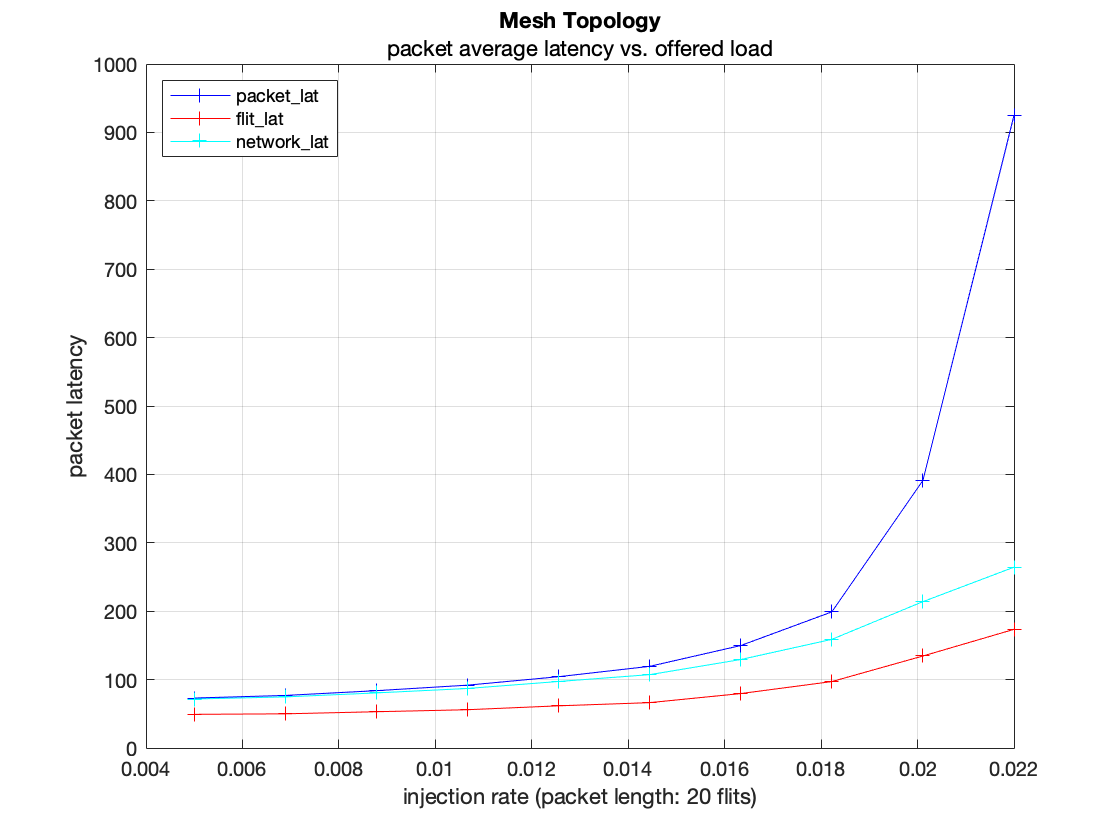
\includegraphics[width=0.45\textwidth]{Images/chap2/mesh_uniform/mesh_dor.png}
    }
    \subfigure[valiant]{
    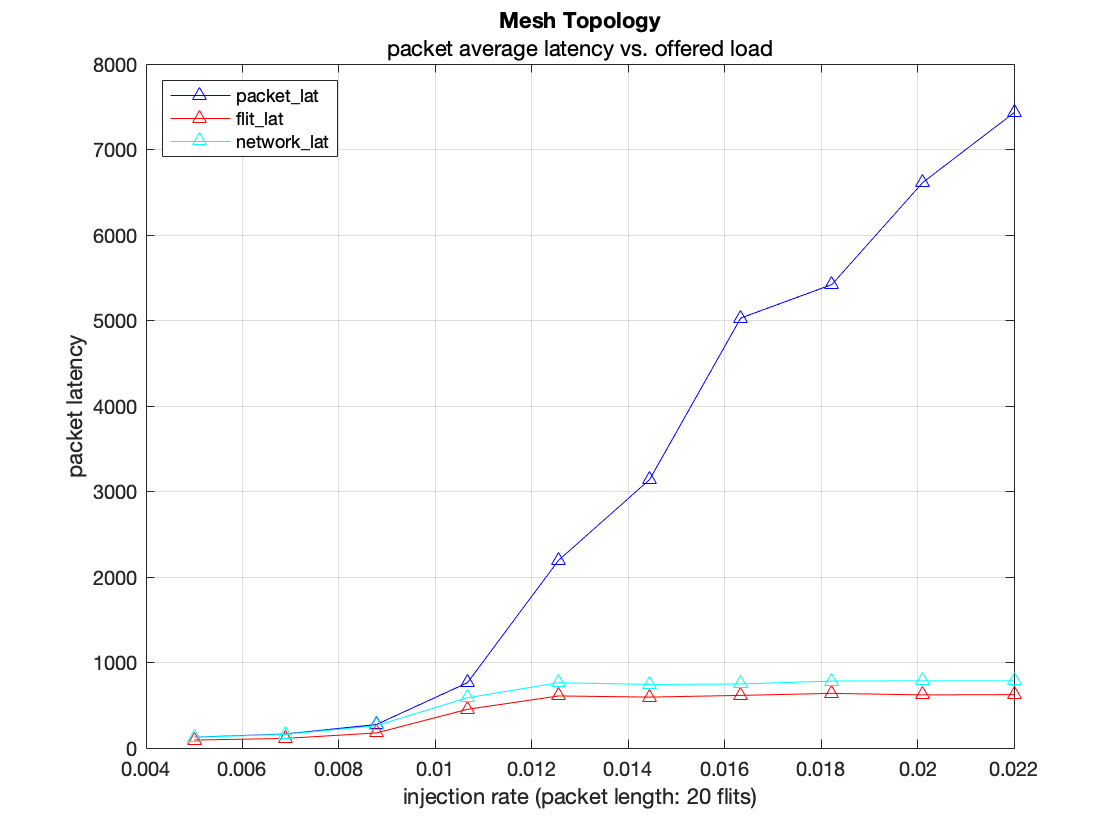
\includegraphics[width=0.45\textwidth]{Images/chap2/mesh_uniform/mesh_val.png}
    }
    \subfigure[romm]{
    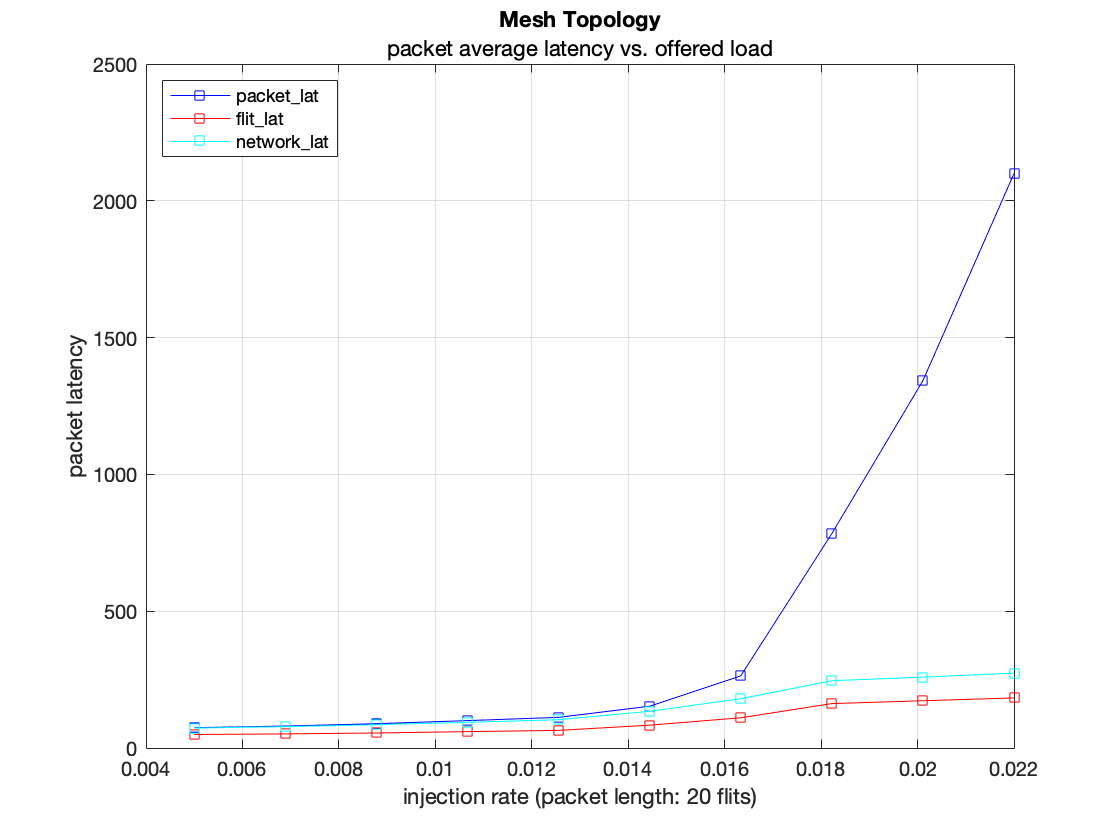
\includegraphics[width=0.45\textwidth]{Images/chap2/mesh_uniform/mesh_romm.png}
    }
    \subfigure[minimal adaptive]{
    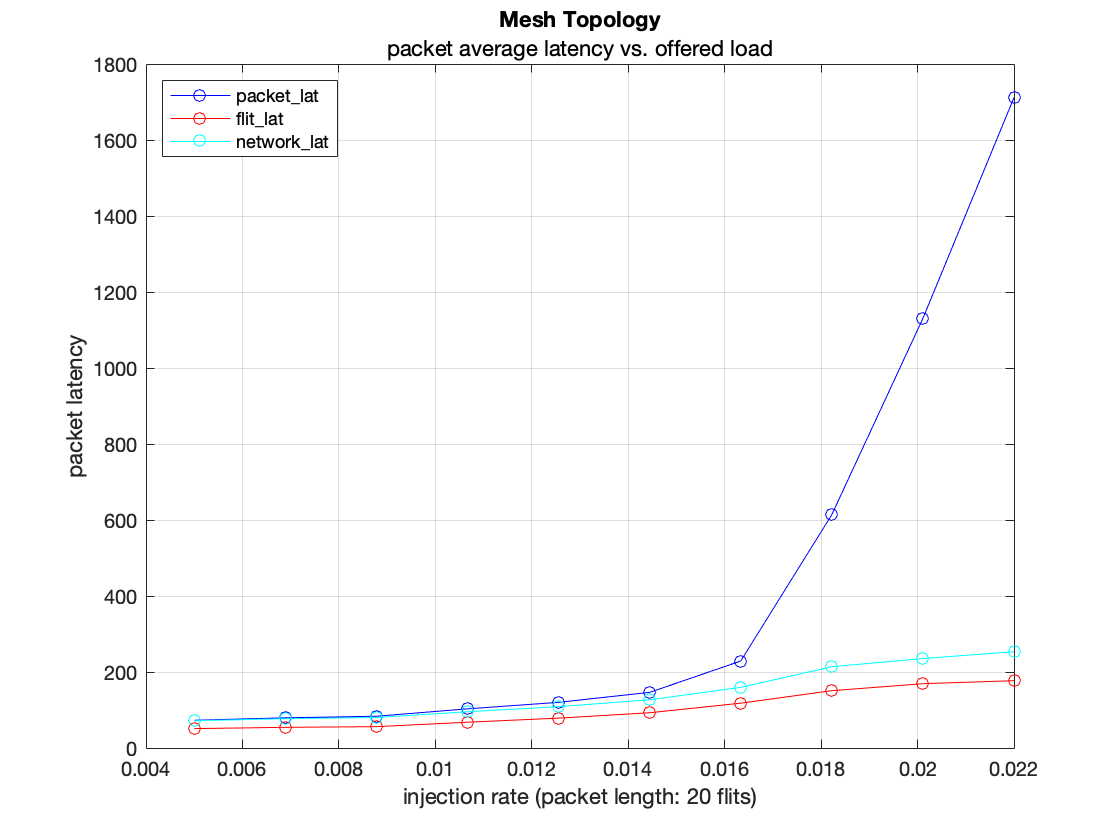
\includegraphics[width=0.45\textwidth]{Images/chap2/mesh_uniform/mesh_min.png}
    }
    \caption{Simulation results of Mesh topology with uniform traffic}
    \label{fig:mesh_uniform}
\end{figure}


\begin{figure}[H]
    \centering
    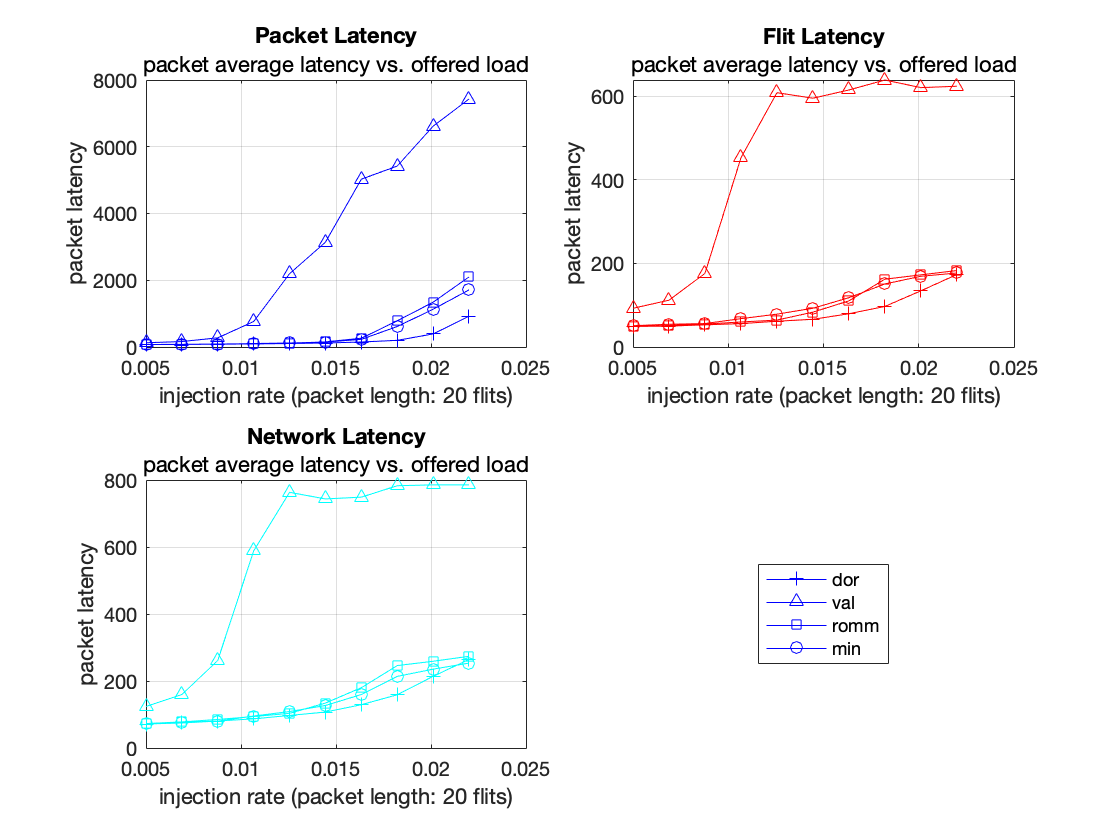
\includegraphics[width=0.9\textwidth]{Images/chap2/mesh_uniform/mesh_comparison.png}
    \caption{Latency comparison of 4 traffic patterns}
    \label{fig:com_mesh_uniform}
\end{figure}



\subsection{Torus(ary8,dim2)}

The second simulation is based on 'torus' topology and 'uniform' traffic pattern to test 3 kinds of different routing algorithms.
\subsubsection{Simulation parameters setup}
The \textbf{basic routing parameters} below are fixed during the whole simulation process:\\
Packet size : 20 flits\\
Router delay : 3 cycles\\
Traffic pattern : uniform\\
Simulation type : latency\\
Latency threshold : 20000\\
The default parameters for \textbf{flow control} in 'booksim\_conf.cpp' are: \\
Virtual channel number : 8\\
Buffer size per channel : 8\\
Wait for tail credit : 0\\

* The default \textbf{latency threshold} set in 'booksim\_conf.cpp' is 500 cycles. It is obvious that lots of average packet latency simulation results greater than 500. To make the simulation more reliable, we must get enough simulation results to reflect the features of a routing algorithm. Therefore, we set the value of latency threshold in the simulation process with 20000 to make the simulation stable and get enough data.


\subsubsection{Simulation results}
The simulation results(average packet/flit/network delay) are listed in the table \ref{tab:torus_uniform}. For each routing algorithm, we test 10 different packet injection rates equally spaced ranging from 0.005 to 0.022.

\subsubsection{Dimension Order Routing Algorithm}
\label{sec:torus_dor}
The simulation results with torus topology under the same traffic pattern and packet injection rates are listed in the table \ref{tab:torus_uniform}. It is obvious that the average packet delay for different packet injection rates with DOR routing algorithm all better than the performance in mesh topology. The key reason is that, compared to the mesh topology, the torus topology links the edge nodes in the mesh topology. Previously, the diameter of the topology is $2*(sqrt(N)-1)$. In torus topology, the diameter is $sqrt(N)$.

\subsubsection{Valiant Randomized Algorithm}
The performance of VAL in torus is also better than in mesh topology with the same reason described above. There is an abnormal simulation result in table \ref{tab:torus_uniform} marked in yellow. The original injection rate should be 0.0201 since the injection rates are equally spaced ranging from 0.005 to 0.022. However, with injection rate of 0.0201, it will always cause deadlock and cannot perform the whole simulation process. The same outcome to the injection rate of 0.0202. So the injection rate 0.0203 marked in yellow is an alternative here.

\subsubsection{Minimal Adaptive Routing Algorithm}
The simulation results with minimal adaptive routing algorithm in torus topology are also better than in mesh topology with the same reason described in \ref{sec:torus_dor}.

The performance of the MIN-ADAPT routing algorithm in torus topology is better than VAL, whilst worse than DOR. Although MIN-ADAPT routing algorithm considers the states of the network, it cannot guarantee always chosing the shortest path from source to destination.

\subsubsection{Simulation Results and Analysis}
\label{sec:torus_uniform_results}
% Please add the following required packages to your document preamble:
% \usepackage[table,xcdraw]{xcolor}
% If you use beamer only pass "xcolor=table" option, i.e. \documentclass[xcolor=table]{beamer}
\begin{longtable}[H]{llllll}
\centering
\label{tab:torus_uniform}
\textbf{topology} &
  \textbf{\begin{tabular}[c]{@{}l@{}}routing\\ \_algorithm\end{tabular}} &
  \textbf{\begin{tabular}[c]{@{}l@{}}injection\\ \_rate\end{tabular}} &
  \textbf{\begin{tabular}[c]{@{}l@{}}average\\ \_packet\\ \_delay\end{tabular}} &
  \textbf{\begin{tabular}[c]{@{}l@{}}average\\ \_network\\ \_latency\end{tabular}} &
  \textbf{\begin{tabular}[c]{@{}l@{}}average\\ \_flit\\ \_delay\end{tabular}} \\ \hline
\endfirsthead %以上是最前的表头
\multicolumn{6}{c}{}\\

\textbf{topology} &
  \textbf{\begin{tabular}[c]{@{}l@{}}routing\\ \_algorithm\end{tabular}} &
  \textbf{\begin{tabular}[c]{@{}l@{}}injection\\ \_rate\end{tabular}} &
  \textbf{\begin{tabular}[c]{@{}l@{}}average\\ \_packet\\ \_delay\end{tabular}} &
  \textbf{\begin{tabular}[c]{@{}l@{}}average\\ \_network\\ \_latency\end{tabular}} &
  \textbf{\begin{tabular}[c]{@{}l@{}}average\\ \_flit\\ \_delay\end{tabular}} \\ \hline
\endhead %以上是换页后的表头,如未换页,并不会显示
\hline
\multicolumn{6}{r}{Continue…}\\
\endfoot %以上是前页的表尾,如未换页,并不会显示。
\hline
\endlastfoot%以上选填最后也的表尾。一般不填
torus(ary8,dim2) & dor        & 0.005                          & 66.7399 & 65.0149 & 42.5716 \\
torus(ary8,dim2) & dor        & 0.0069                         & 69.5791 & 67.1535 & 43.3476 \\
torus(ary8,dim2) & dor        & 0.0088                         & 74.6169 & 70.6552 & 45.1903 \\
torus(ary8,dim2) & dor        & 0.0107                         & 76.7209 & 72.1913 & 46.1854 \\
torus(ary8,dim2) & dor        & 0.0126                         & 83.0781 & 76.5032 & 47.8748 \\
torus(ary8,dim2) & dor        & 0.0144                         & 88.2678 & 79.2485 & 49.4006 \\
torus(ary8,dim2) & dor        & 0.0162                         & 95.1119 & 83.882  & 51.6748 \\
torus(ary8,dim2) & dor        & 0.0182                         & 105.513 & 89.2365 & 54.2422 \\
torus(ary8,dim2) & dor        & 0.0201                         & 118.494 & 96.4839 & 58.2716 \\
torus(ary8,dim2) & dor        & 0.022                          & 139.122 & 104.441 & 62.9165 \\ \hline
torus(ary8,dim2) & val        & 0.005                          & 107.974 & 106.021 & 78.5071 \\
torus(ary8,dim2) & val        & 0.0069                         & 120.072 & 116.528 & 84.0434 \\
torus(ary8,dim2) & val        & 0.0088                         & 135.254 & 130.466 & 91.0194 \\
torus(ary8,dim2) & val        & 0.0107                         & 157.945 & 149.038 & 102.686 \\
torus(ary8,dim2) & val        & 0.0126                         & 195.304 & 179.965 & 121.86  \\
torus(ary8,dim2) & val        & 0.0144                         & 272.25  & 226.084 & 155.958 \\
torus(ary8,dim2) & val        & 0.0162                         & 658.898 & 332.127 & 245.099 \\
torus(ary8,dim2) & val        & 0.0182                         & 1301.86 & 366.269 & 274.249 \\
torus(ary8,dim2) & val        & \cellcolor[HTML]{FFFF00}0.0203 & 2276.21 & 365.761 & 277.312 \\
torus(ary8,dim2) & val        & 0.022                          & 3064.75 & 362.109 & 279.278 \\ \hline
torus(ary8,dim2) & min\_adapt & 0.005                          & 67.0736 & 65.2945 & 43.9873 \\
torus(ary8,dim2) & min\_adapt & 0.0069                         & 69.3613 & 67.0838 & 45.1162 \\
torus(ary8,dim2) & min\_adapt & 0.0088                         & 75.7793 & 71.8472 & 48.9873 \\
torus(ary8,dim2) & min\_adapt & 0.0107                         & 82.82   & 76.9492 & 52.1749 \\
torus(ary8,dim2) & min\_adapt & 0.0126                         & 91.8262 & 82.0425 & 56.353  \\
torus(ary8,dim2) & min\_adapt & 0.0144                         & 108.177 & 90.2746 & 63.1311 \\
torus(ary8,dim2) & min\_adapt & 0.0162                         & 144.896 & 100.749 & 71.3917 \\
torus(ary8,dim2) & min\_adapt & 0.0182                         & 291.051 & 120.425 & 87.2741 \\
torus(ary8,dim2) & min\_adapt & 0.0201                         & 803.945 & 135.229 & 99.242  \\
torus(ary8,dim2) & min\_adapt & 0.022                          & 1535.8  & 141.041 & 103.491 \\ \hline
\end{longtable}



The blue lines in all the figures \ref{fig:torus_uniform}, \ref{fig:com_torus_uniform} depicts the change of the average packet delay against offered load. According to the first sub-figure in the figure \ref{fig:com_torus_uniform}, we can know that the performance of the DOR routing algorithm in such a torus(8-ary, 2-dim) topology with uniform traffic patterns is better than all the other three routing algorithms(VAL, MIN-ADAPT).

The data in Tab. \ref{tab:torus_uniform} marked in yellow is initially should be 0.0201; however, the simulation results with an injection rate of 0.0201(same results with 0.0202) will always lead to a deadlock. Thus, the injection rates intervals between 0.0182 and 0.022 are not distributed evenly.

\begin{figure}[H]
    \centering
    \subfigure[dimension order]{
    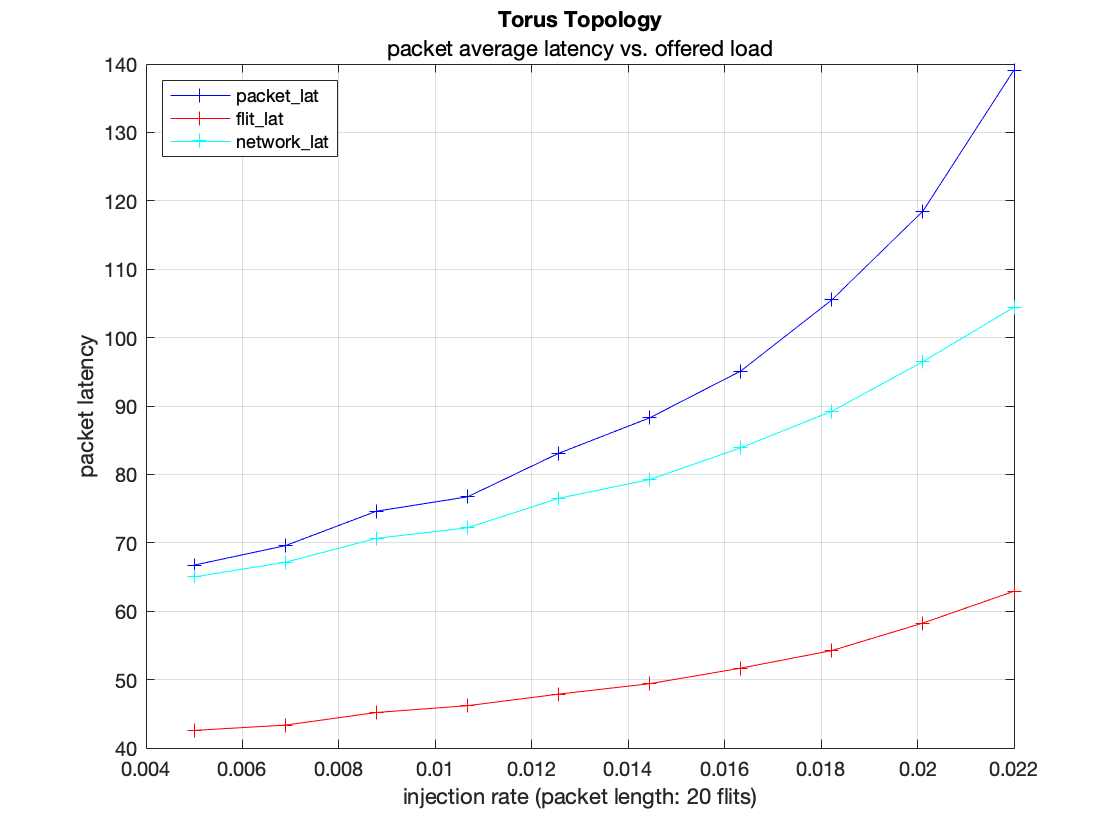
\includegraphics[width=0.45\textwidth]{Images/chap2/torus_uniform/torus_dor.png}
    %\caption{fig1}
    }
    \subfigure[valiant]{
    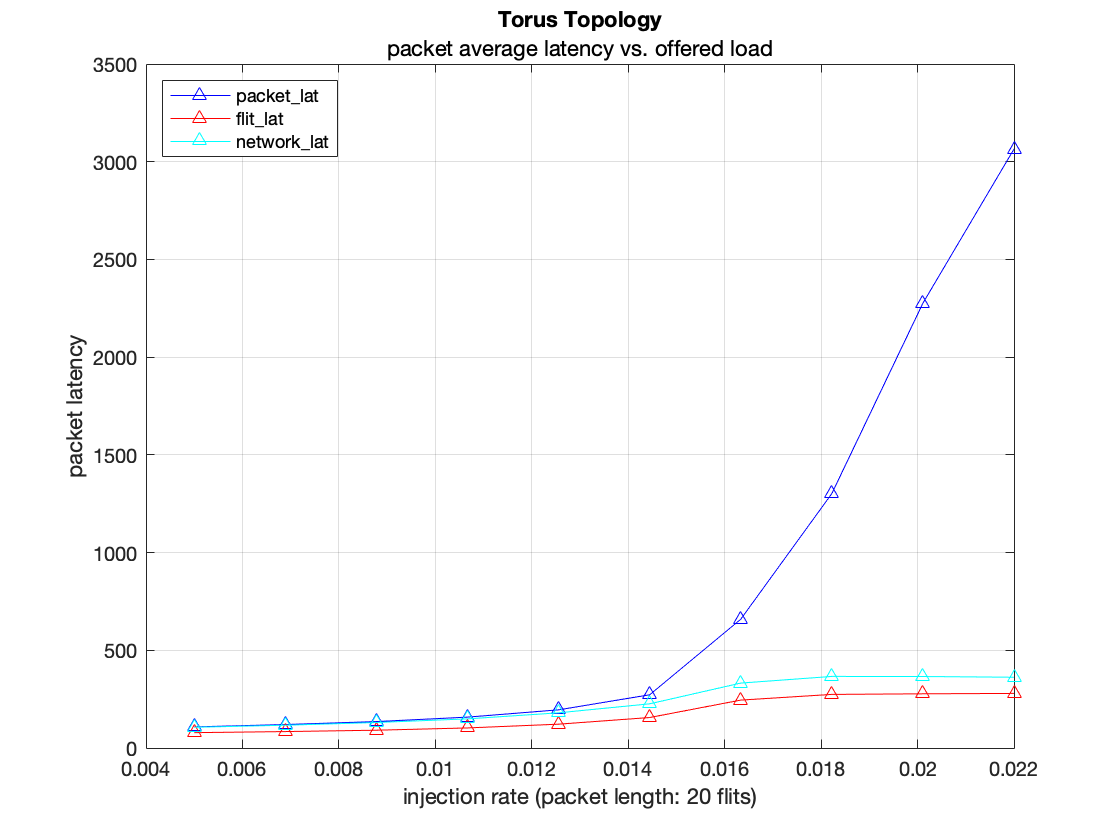
\includegraphics[width=0.45\textwidth]{Images/chap2/torus_uniform/torus_val.png}
    }
    \subfigure[minimal adaptive]{
    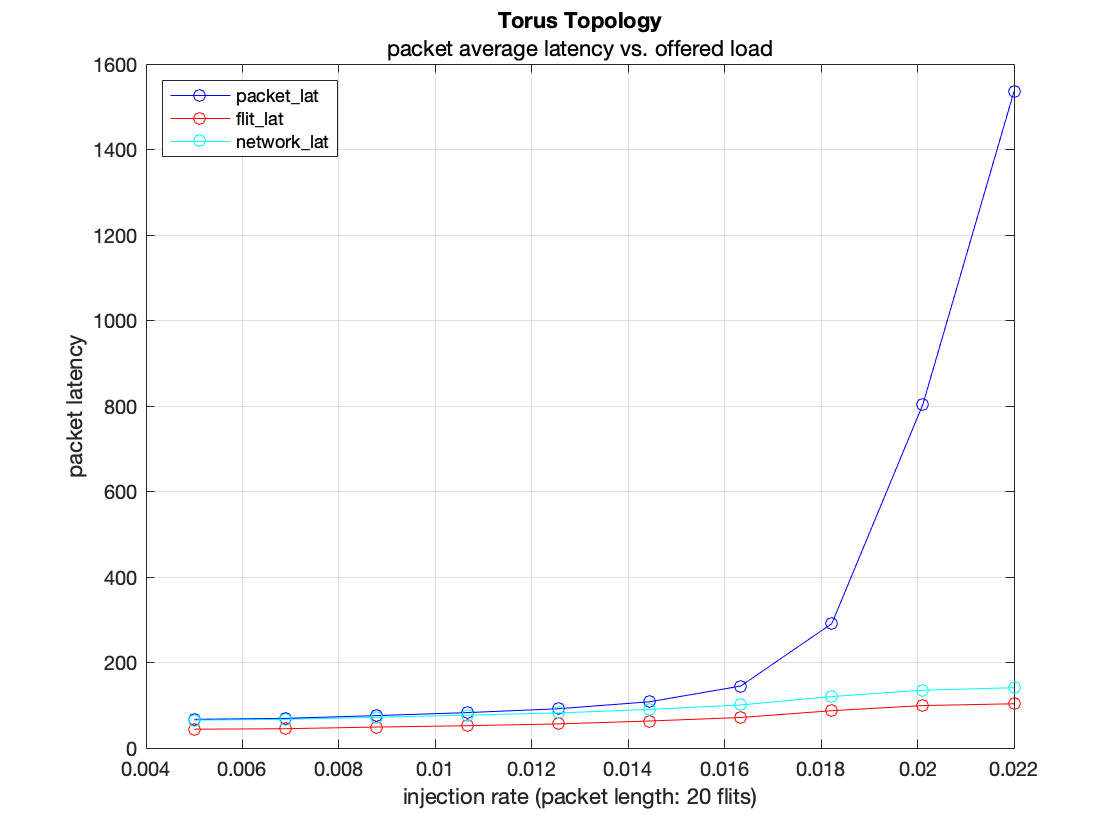
\includegraphics[width=0.45\textwidth]{Images/chap2/torus_uniform/torus_min.png}
    }
    \caption{Simulation results of Torus topology with uniform traffic}
    \label{fig:torus_uniform}
\end{figure}


\begin{figure}[H]
    \centering
    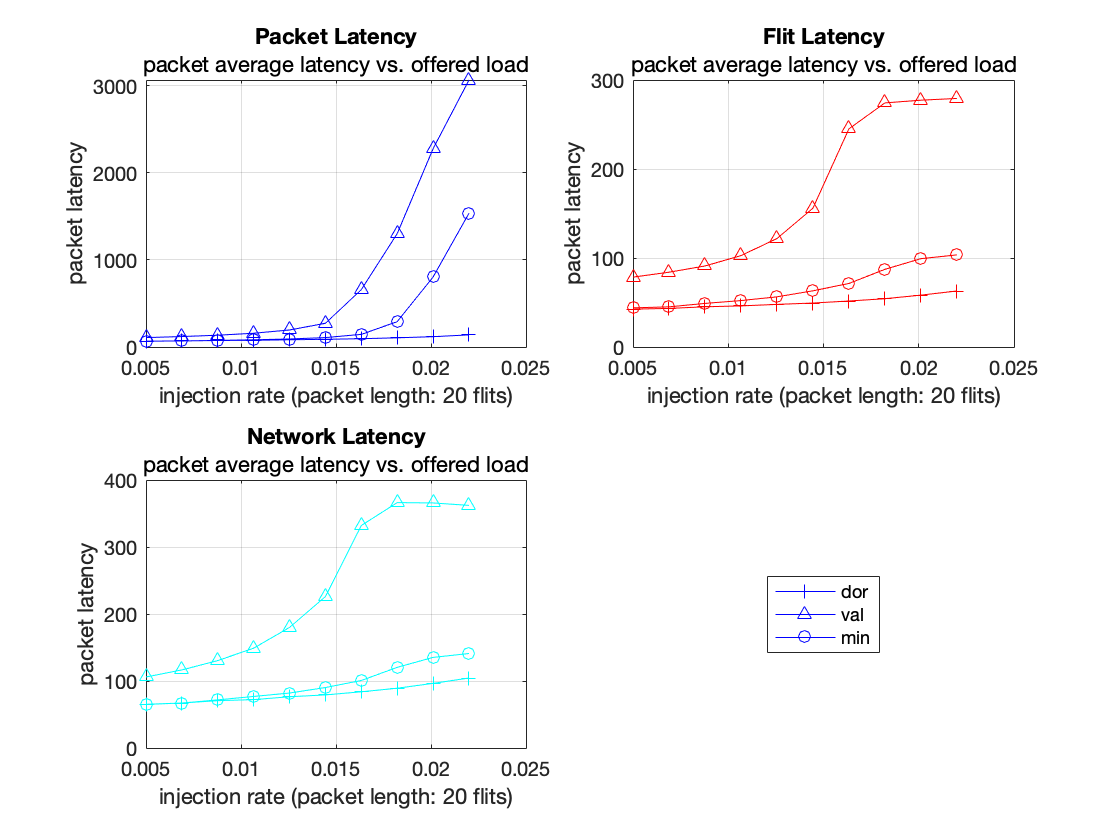
\includegraphics[width=0.9\textwidth]{Images/chap2/torus_uniform/torus_comparison.png}
    \caption{Latency comparison of 4 traffic patterns}
    \label{fig:com_torus_uniform}
\end{figure}

\subsection{Performance Comparison and Analysis}

\begin{figure}[H]
    \centering
    \subfigure[dimension order]{
    \label{com_dor_uniform}
    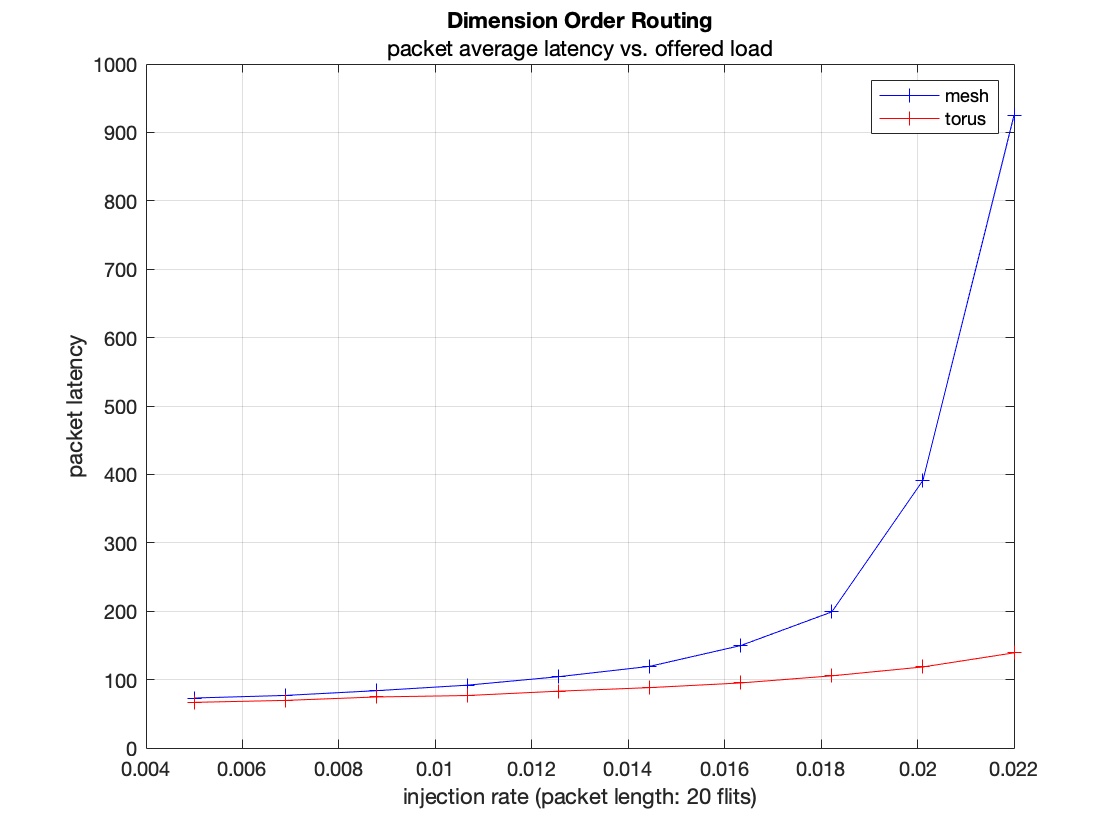
\includegraphics[width=0.45\textwidth]{Images/chap2/Comparison/Com_dor_uniform.png}
    %\caption{fig1}
    }
    \subfigure[valiant]{
    \label{com_val_uniform}
    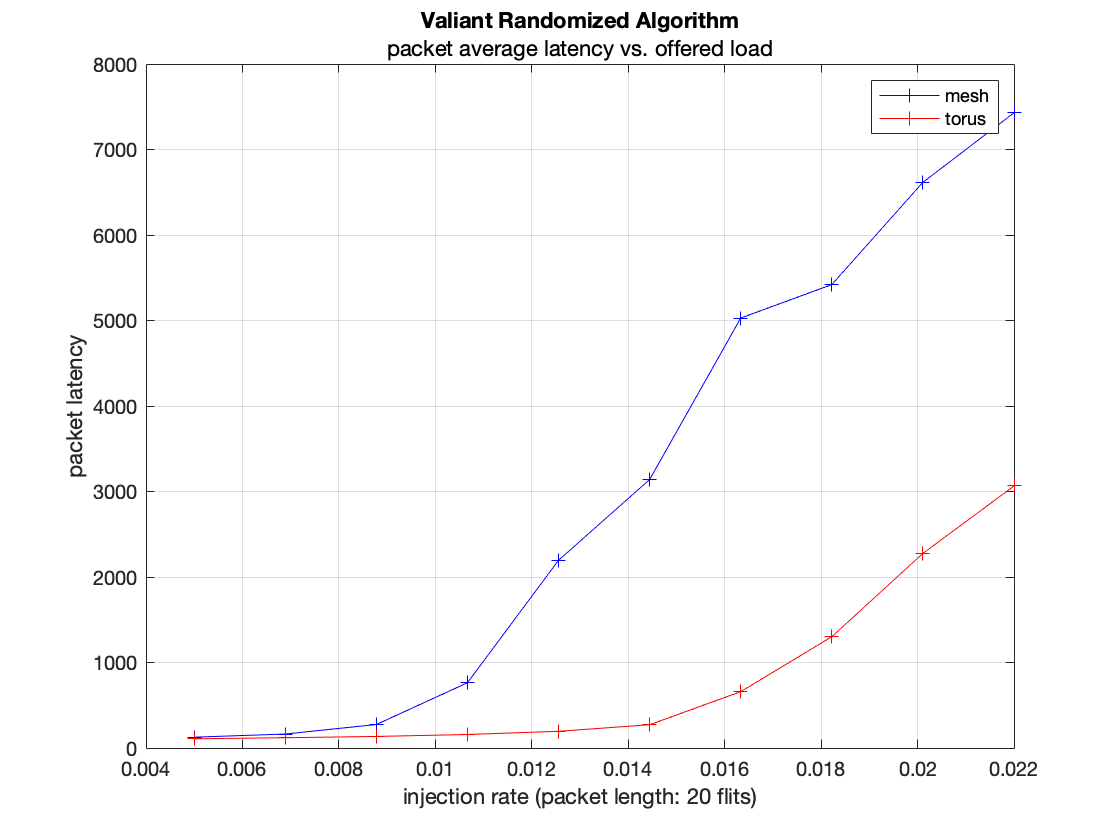
\includegraphics[width=0.45\textwidth]{Images/chap2/Comparison/Com_val_uniform.png}
    }
    \subfigure[minimal adaptive]{
    \label{com_min_uniform}
    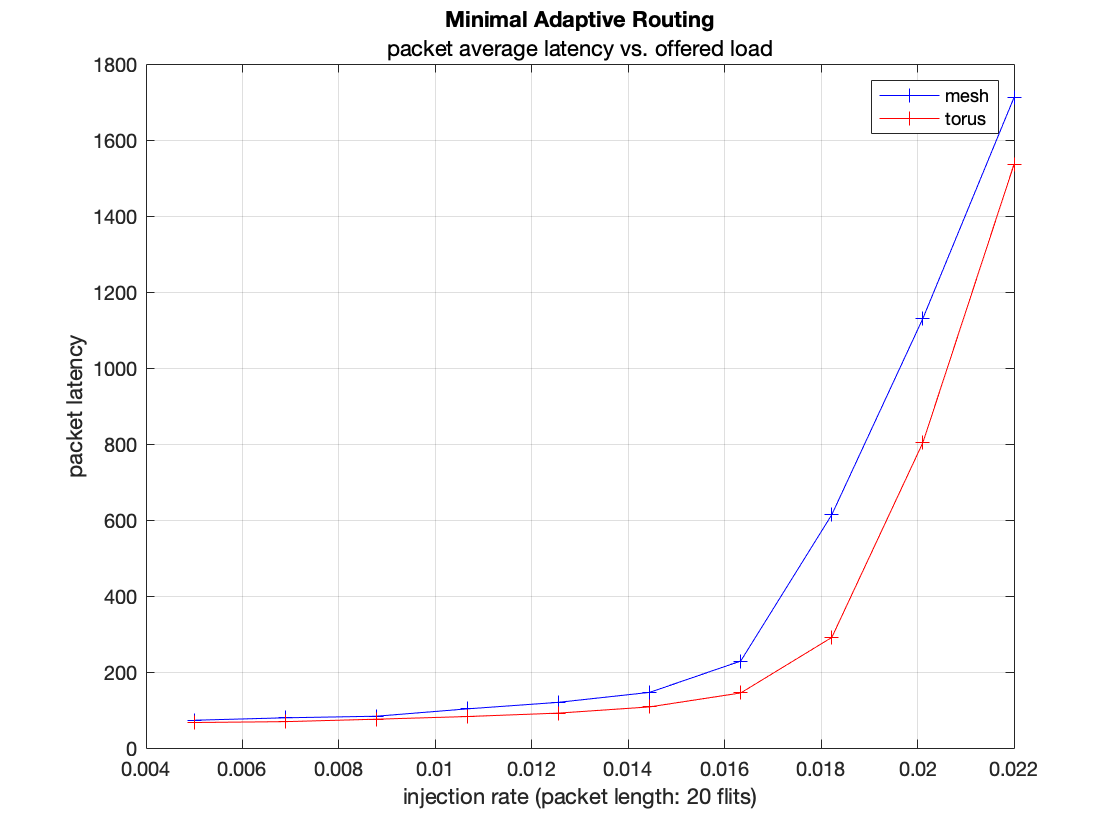
\includegraphics[width=0.45\textwidth]{Images/chap2/Comparison/Com_min_uniform.png}
    }
    \caption{Comparison under 'Uniform' traffic pattern}
    \label{fig:com_uniform}
\end{figure}

The figure \ref{fig:com_uniform} compared the mesh and torus with different algorithms(DOR, VAL, MIN-ADAPT) separately. The average packet delay in all the sub-figures of Torus topology(red curve) always below the average packet delay of Mesh topology(blue curve). The difference of the average packet delay of these two topologies is quite small, but with the injection rate increasing, the difference also increases.
From the analysis above, we can draw the conclusion that: under the uniform traffic pattern, no matter we use which routing algorithm in the network, the performance of Torus topology always better than Mesh topology.
DOR routing algorithm is the suitable for both mesh and torus topologies under uniform traffic pattern.














\section{Use “Tornado” traffic pattern}

Evaluate all the routing algorithms to get plots of average latency vs. offered load. Compare the performance of the two topologies and explain the possible reasons.

\subsection{Mesh(ary8,dim2)}

The first simulation is based on 'mesh' topology and 'tornado' traffic pattern to test 4 kinds of different routing algorithms(DOR, VAL, ROMM, MIN-ADAPT).
\subsubsection{Simulation parameters setup}
The \textbf{basic routing parameters} below are fixed during the whole simulation process:\\
Packet size : 20 flits\\
Router delay : 3 cycles\\
Traffic pattern : tornado\\
Simulation type : latency\\
Latency threshold : 20000\\
The default parameters for \textbf{flow control} in 'booksim\_conf.cpp' are: \\
Virtual channel number : 8\\
Buffer size per channel : 8\\
Wait for tail credit : 0\\

* The default \textbf{latency threshold} set in 'booksim\_conf.cpp' is 500 cycles. It is obvious that lots of average packet latency simulation results greater than 500. To make the simulation more reliable, we must get enough simulation results to reflect the features of a routing algorithm. Therefore, we set the value of latency threshold in the simulation process with 20000 to make the simulation stable and get enough data.
\subsubsection{Simulation results}

The simulation results(average packet/flit/network delay) are listed in the table \ref{tab:mesh_tornado}. For each routing algorithm, we test 10 different packet injection rates equally spaced ranging from 0.005 to 0.022.


\subsubsection{Dimension Order Routing Algorithm}
The first ten rows in the table \ref{tab:mesh_tornado} is the simulation results of dimension order routing algorithm(DOR). The average packet delay is increased non-linearly. The lowest average packet delay is 92, and the corresponding injection rate is 0.005. The highest average packet delay is 4574, and the corresponding injection rate is 0.022. DOR is a basic routing algorithm in such an interconnection network topology.

\subsubsection{Valiant Randomized Algorithm}
The next ten rows following dimension order algorithm is simulated with Valiant Randomized routing algorithm(VAL). Similar to the simulation results of DOR, the increment of the average packet delay is non-linear. The value of the average packet delay exceeds 500 with the injection rate of 0.0107. It is obvious that under 'mesh' topology and 'tornado' traffic pattern, the performance of DOR algorithm is much better than the VAL. Compared with DOR, VAL will firstly select an intermediate node randomly. Packets will go through this node and then be transmitted to the destination. The detour in the VAL causes the performance of VAL worse than DOR.

\subsubsection{The Randomized Minimal Algorithm}
The randomized minimal algorithm(ROMM) is a minimal version of Valiant's algorithm. So the performance of the ROMM is better than VAL. However, its performance still is not better than DOR. The lowest value of average packet delay is 96, and the highest value of average packet value is 8106. For the injection rates lower than 0,0126, the corresponding average packet delays all below 500.

\subsubsection{Minimal Adaptive Routing Algorithm}
This routing algorithm is a different class compared to the three routing algorithm above. All the three algorithms(DOR, VAL, ROMM) above are deterministic, which means that routes choosing for packets without considering any information about the network present state. Deterministic algorithms are a subset of oblivious algorithms. All the packets from the same source and destination pairs will always choose the same path. In adaptive algorithms, the state of the network is incorporated in making routing decision to adapt to network state such as network congestion. the decision of the routes depending on the states(node, link, length of queues, historical channel load information) of the network.

The last ten rows in the table \ref{tab:mesh_tornado} is the simulation results of the minimal adaptive routing algorithm(MIN-ADAPT). The performance of the MIN-ADAPT routing algorithm is better than ROMM and VAL, whilst worse than DOR. Although MIN-ADAPT routing algorithm considers the states of the network, it cannot guarantee always chosing the shortest path from source to destination.



\subsubsection{Simulation Results and Analysis}
\label{sec:mesh_tornado_results}
% Please add the following required packages to your document preamble:
% \usepackage[table,xcdraw]{xcolor}
% If you use beamer only pass "xcolor=table" option, i.e. \documentclass[xcolor=table]{beamer}
\begin{longtable}[H]{llllll}
\centering
\label{tab:mesh_tornado}
\textbf{topology} &
  \textbf{\begin{tabular}[c]{@{}l@{}}routing\\ \_algorithm\end{tabular}} &
  \textbf{\begin{tabular}[c]{@{}l@{}}injection\\ \_rate\end{tabular}} &
  \textbf{\begin{tabular}[c]{@{}l@{}}average\\ \_packet\\ \_delay\end{tabular}} &
  \textbf{\begin{tabular}[c]{@{}l@{}}average\\ \_network\\ \_latency\end{tabular}} &
  \textbf{\begin{tabular}[c]{@{}l@{}}average\\ \_flit\\ \_delay\end{tabular}} \\ \hline
\endfirsthead %以上是最前的表头
\multicolumn{6}{c}{}\\

\textbf{topology} &
  \textbf{\begin{tabular}[c]{@{}l@{}}routing\\ \_algorithm\end{tabular}} &
  \textbf{\begin{tabular}[c]{@{}l@{}}injection\\ \_rate\end{tabular}} &
  \textbf{\begin{tabular}[c]{@{}l@{}}average\\ \_packet\\ \_delay\end{tabular}} &
  \textbf{\begin{tabular}[c]{@{}l@{}}average\\ \_network\\ \_latency\end{tabular}} &
  \textbf{\begin{tabular}[c]{@{}l@{}}average\\ \_flit\\ \_delay\end{tabular}} \\ \hline
\endhead %以上是换页后的表头,如未换页,并不会显示
\hline
\multicolumn{6}{r}{Continue…}\\
\endfoot %以上是前页的表尾,如未换页,并不会显示。
\hline
\endlastfoot%以上选填最后也的表尾。一般不填
mesh(ary8,dim2) & dor & 0.005  & 92.5512 & 90.9669 & 65.8955 \\
mesh(ary8,dim2) & dor                         & 0.0069 & 98.7774 & 96.2007 & 68.3627 \\
mesh(ary8,dim2) & dor                         & 0.0088 & 117.208 & 113.057 & 77.0379 \\
mesh(ary8,dim2) & dor                         & 0.0107 & 139.696 & 131.427 & 87.5752 \\
mesh(ary8,dim2) & dor                         & 0.0126 & 219.069 & 195.073 & 129.456 \\
mesh(ary8,dim2) & dor                         & 0.0144 & 471.793 & 308.206 & 214.884 \\
mesh(ary8,dim2) & dor                         & 0.0162 & 1399.5  & 445.489 & 353.935 \\
mesh(ary8,dim2) & dor                         & 0.0182 & 2294.67 & 523.546 & 431.162 \\
mesh(ary8,dim2) & dor                         & 0.0201 & 3685.97 & 562.134 & 456.579 \\
mesh(ary8,dim2) & dor                         & 0.022  & 4574.78 & 569.106 & 461.14  \\ \hline
mesh(ary8,dim2) & val                         & 0.005  & 126.226 & 124.342 & 93.5684 \\
mesh(ary8,dim2) & val                         & 0.0069 & 156.676 & 153.348 & 108.156 \\
mesh(ary8,dim2) & val                         & 0.0088 & 285.179 & 270.562 & 180.599 \\
mesh(ary8,dim2) & val                         & 0.0107 & 747.549 & 575.838 & 442.555 \\
mesh(ary8,dim2) & val                         & 0.0126 & 2053.08 & 725.558 & 640.968 \\
mesh(ary8,dim2) & val                         & 0.0144 & 3814.45 & 830.045 & 686.359 \\
mesh(ary8,dim2) & val                         & 0.0162 & 6192.3  & 856.751 & 701.208 \\
mesh(ary8,dim2) & val                         & 0.0182 & 8041.86 & 892.967 & 692.578 \\
mesh(ary8,dim2) & val                         & 0.0201 & 7796    & 870.164 & 729.27  \\
mesh(ary8,dim2) & val                         & 0.022  & 8569.72 & 856.703 & 714.446 \\ \hline
mesh(ary8,dim2) & romm                        & 0.005  & 96.4438 & 94.857  & 67.6557 \\
mesh(ary8,dim2) & romm                        & 0.0069 & 112.702 & 109.95  & 74.673  \\
mesh(ary8,dim2) & romm                        & 0.0088 & 168.245 & 159.831 & 103.616 \\
mesh(ary8,dim2) & romm                        & 0.0107 & 440.438 & 272.12  & 215.058 \\
mesh(ary8,dim2) & romm                        & 0.0126 & 1325.87 & 443.626 & 349.825 \\
mesh(ary8,dim2) & romm                        & 0.0144 & 3148.01 & 522.839 & 407.701 \\
mesh(ary8,dim2) & romm                        & 0.0162 & 4539.88 & 551.965 & 447.395 \\
mesh(ary8,dim2) & romm                        & 0.0182 & 5478.99 & 546.734 & 446.799 \\
mesh(ary8,dim2) & romm                        & 0.0201 & 7106.34 & 552.425 & 459.937 \\
mesh(ary8,dim2) & romm                        & 0.022  & 8106.32 & 579.571 & 460.133 \\ \hline
mesh(ary8,dim2) & min\_adapt                  & 0.005  & 92.4276 & 91.0017 & 69.6105 \\
mesh(ary8,dim2) & min\_adapt                  & 0.0069 & 101.992 & 99.497  & 74.1709 \\
mesh(ary8,dim2) & min\_adapt                  & 0.0088 & 124.28  & 118.963 & 88.0493 \\
mesh(ary8,dim2) & min\_adapt                  & 0.0107 & 157.429 & 148.367 & 107.914 \\
mesh(ary8,dim2) & min\_adapt                  & 0.0126 & 278.497 & 234.037 & 175.002 \\
mesh(ary8,dim2) & min\_adapt                  & 0.0144 & 775.582 & 349.928 & 301.309 \\
mesh(ary8,dim2) & min\_adapt                  & 0.0162 & 1888.02 & 477.1   & 375.548 \\
mesh(ary8,dim2) & min\_adapt                  & 0.0182 & 3220.62 & 536.745 & 430.401 \\
mesh(ary8,dim2) & min\_adapt                  & 0.0201 & 4601.75 & 606.393 & 457.444 \\
mesh(ary8,dim2) & min\_adapt                  & 0.022  & 6315.09 & 602.46  & 428.54 
\end{longtable}



The blue lines in all the figures \ref{fig:mesh_tornado}, \ref{fig:com_mesh_tornado} depicts the change of the average packet delay against offered load. According to the first sub-figure in the figure \ref{fig:com_mesh_tornado}, we can know that the performance of the DOR routing algorithm in such a mesh(8-ary, 2-dim) topology with uniform traffic pattern better than all the other three routing algorithms(VAL, ROMM, MIN-ADAPT).


\begin{figure}[H]
    \centering
    \subfigure[dimension order]{
    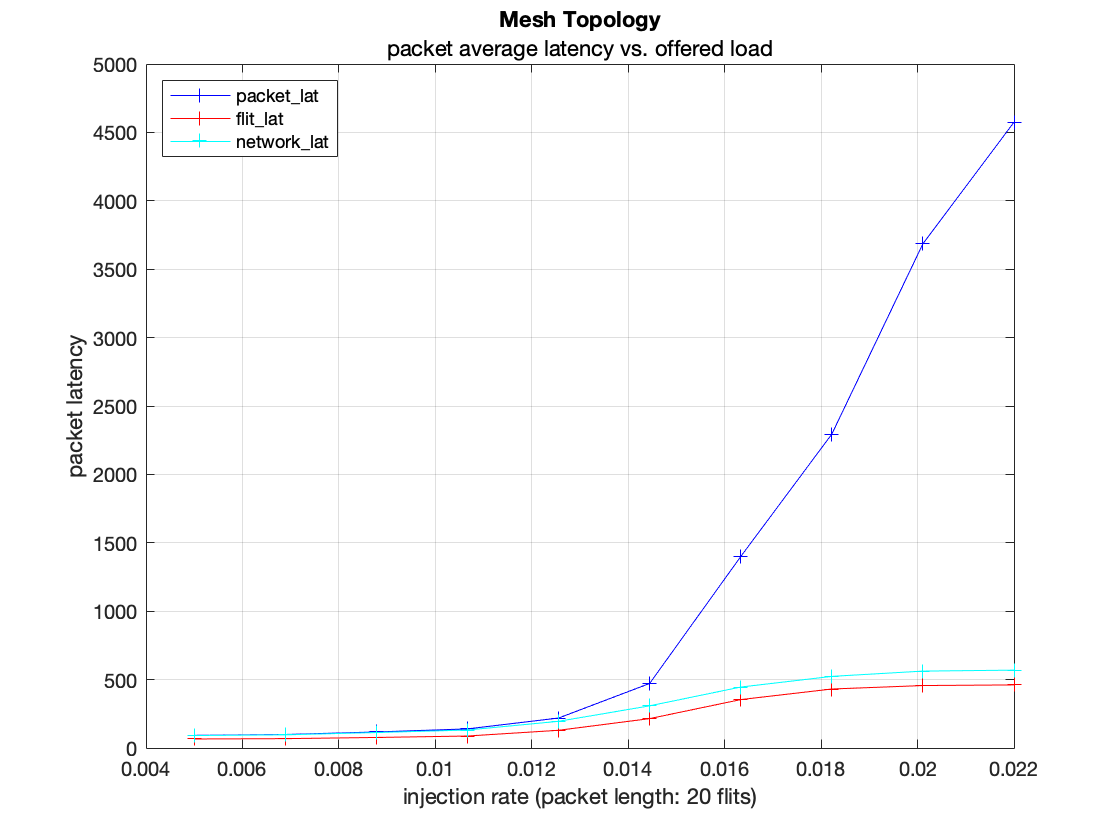
\includegraphics[width=0.45\textwidth]{Images/chap2/mesh_tornado/mesh_dor.png}
    }
    \subfigure[valiant]{
    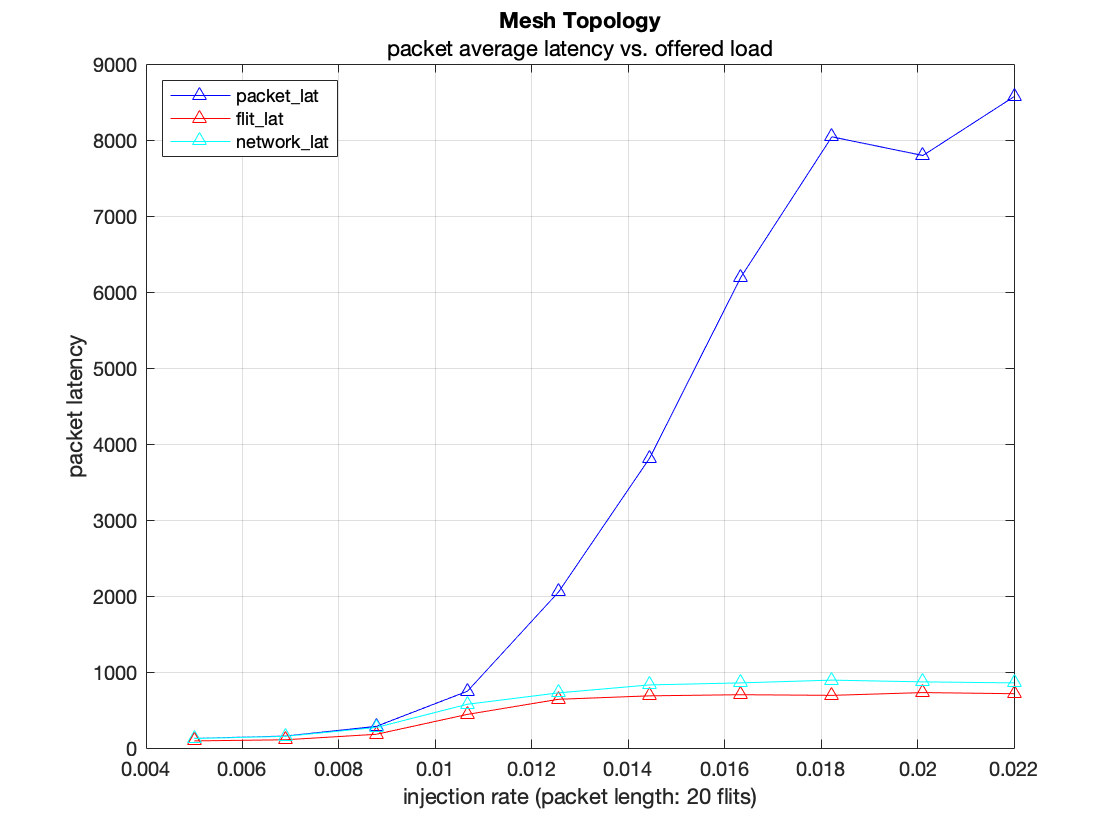
\includegraphics[width=0.45\textwidth]{Images/chap2/mesh_tornado/mesh_val.png}
    }
    \subfigure[romm]{
    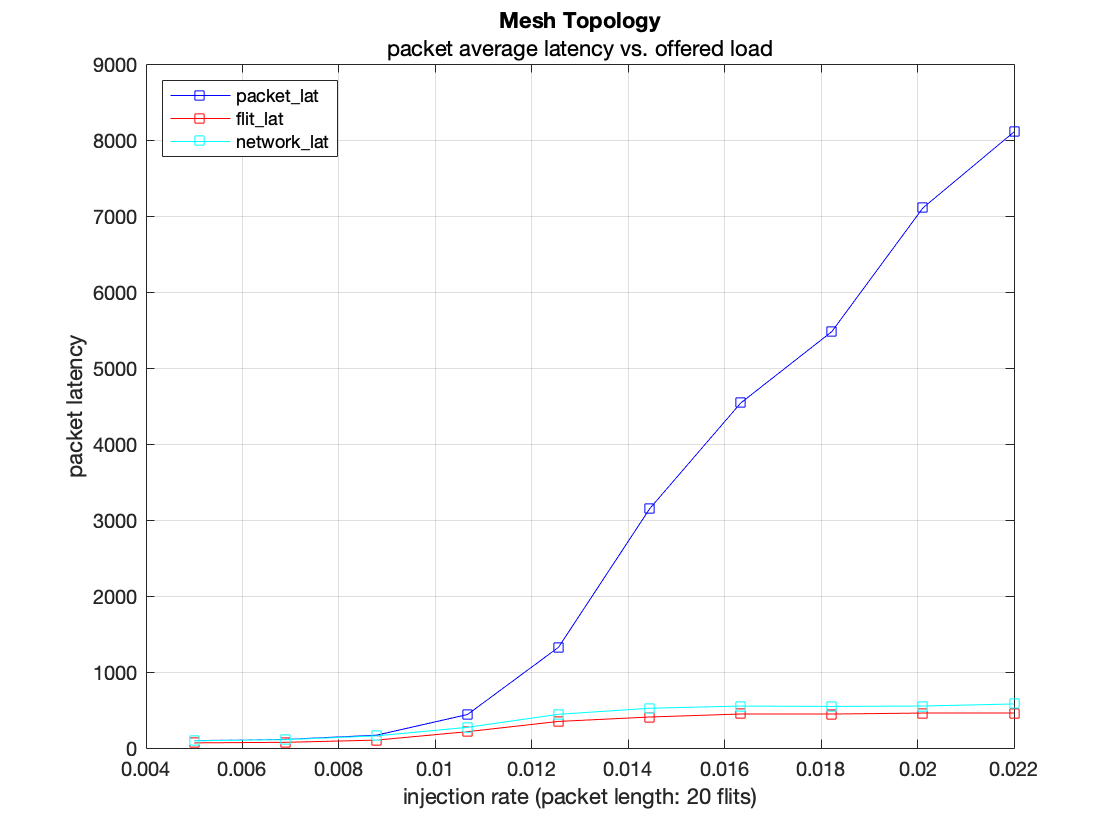
\includegraphics[width=0.45\textwidth]{Images/chap2/mesh_tornado/mesh_romm.png}
    }
    \subfigure[minimal adaptive]{
    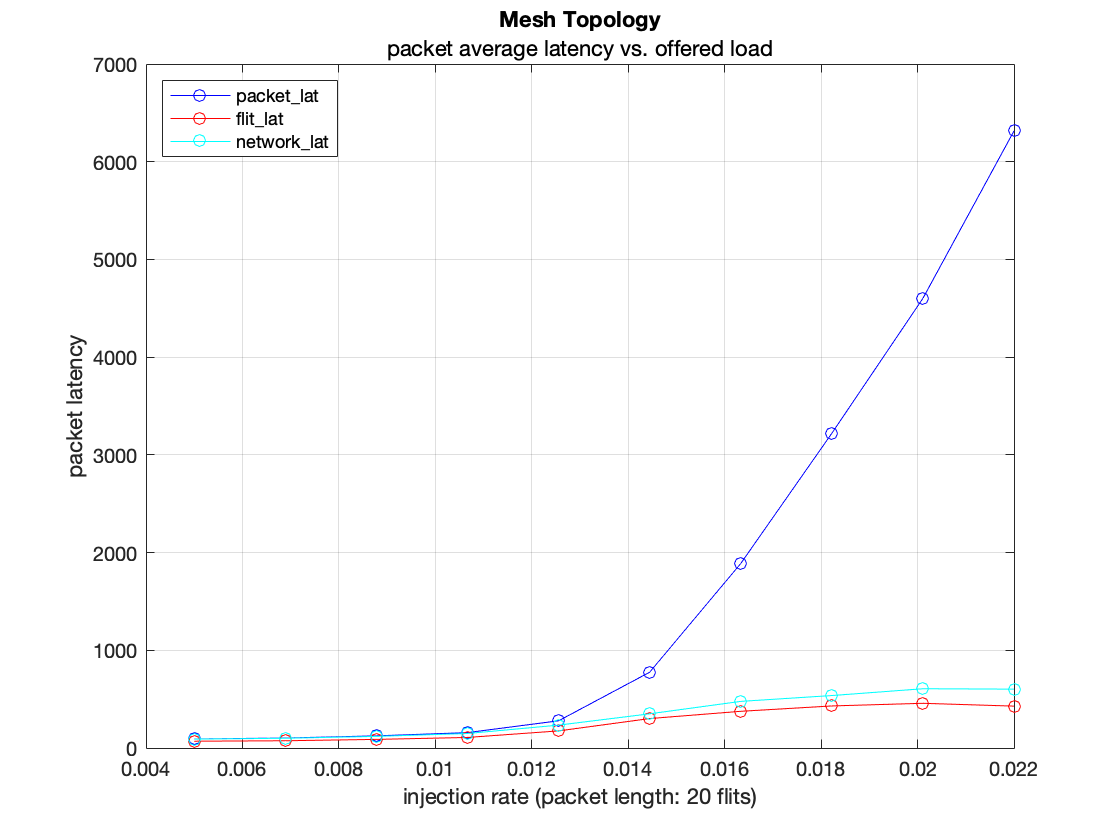
\includegraphics[width=0.45\textwidth]{Images/chap2/mesh_tornado/mesh_min_tornado.png}
    }
    \caption{Simulation results of Mesh topology with uniform traffic}
    \label{fig:mesh_tornado}
\end{figure}


\begin{figure}[H]
    \centering
    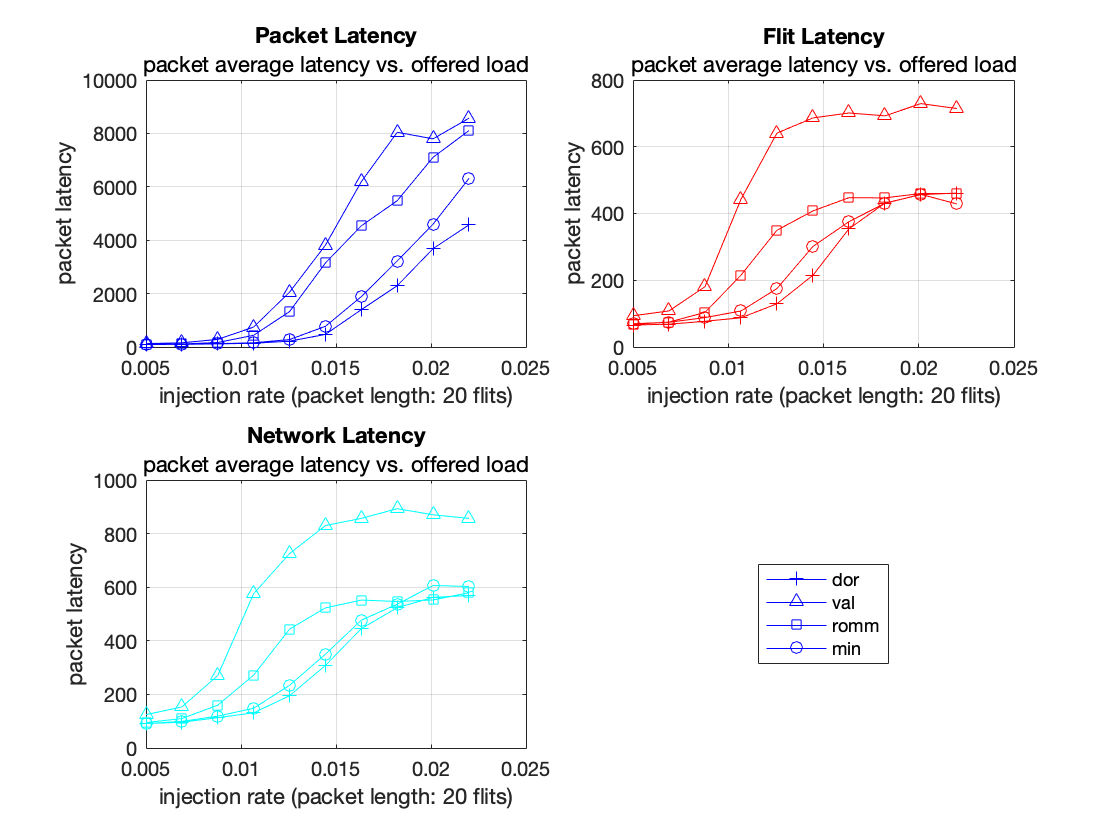
\includegraphics[width=0.9\textwidth]{Images/chap2/mesh_tornado/mesh_comparison_tornado.png}
    \caption{Latency comparison of 4 traffic patterns}
    \label{fig:com_mesh_tornado}
\end{figure}






\subsection{Torus(ary8,dim2)}

The simulation based on 'mesh' topology and 'uniform' traffic pattern for testing 3 kinds of different routing algorithms(DOR, VAL, MIN-ADAPT).
\subsubsection{Simulation parameters setup}
The \textbf{basic routing parameters} below are fixed during the whole simulation process:\\
Packet size : 20 flits\\
Router delay : 3 cycles\\
Traffic pattern : tornado\\
Simulation type : latency\\
Latency threshold : 20000\\
The default parameters for \textbf{flow control} in 'booksim\_conf.cpp' are: \\
Virtual channel number : 8\\
Buffer size per channel : 8\\
Wait for tail credit : 0\\

* The default \textbf{latency threshold} set in 'booksim\_conf.cpp' is 500 cycles. It is obvious that lots of average packet latency simulation results greater than 500. To make the simulation more reliable, we must get enough simulation results to reflect the features of a routing algorithm. Therefore, we set the value of latency threshold in the simulation process with 20000 to make the simulation stable and get enough data.
\subsubsection{Simulation results}

The simulation results(average packet/flit/network delay) are listed in the table \ref{tab:torus_tornado}. For each routing algorithm, we test 10 different packet injection rates equally spaced ranging from 0.005 to 0.022.


\subsubsection{Dimension Order Routing Algorithm}
The first ten rows in the table \ref{tab:torus_tornado} is the simulation results of dimension order routing algorithm(DOR). The average packet delay is increased non-linearly. The lowest average packet delay is 92, and the corresponding injection rate is 0.005. The highest average packet delay is 5043, and the corresponding injection rate is 0.022. DOR is a basic routing algorithm in such an interconnection network topology.

\subsubsection{Valiant Randomized Algorithm}
The next ten rows following dimension order algorithm is simulated with Valiant Randomized routing algorithm(VAL). Similar to the simulation results of DOR, the increment of the average packet delay is non-linear. The value of the average packet delay exceeds 500 with the injection rate of 0.0162. It is obvious that under 'torus' topology and 'tornado' traffic pattern, the performance of VAL algorithm is better than the DOR. Overall, the VAL routing algorithm is suitable for tornado traffic pattern in torus topology.

\subsubsection{Minimal Adaptive Routing Algorithm}
This routing algorithm is a different class compared to the three routing algorithm above. All the three algorithms(DOR, VAL, ROMM) above are deterministic, which means that routes choosing for packets without considering any information about the network present state. Deterministic algorithms are a subset of oblivious algorithms. All the packets from the same source and destination pairs will always choose the same path. In adaptive algorithms, the state of the network is incorporated in making routing decision to adapt to network state such as network congestion. the decision of the routes depending on the states(node, link, length of queues, historical channel load information) of the network.

The last ten rows in the table \ref{tab:torus_tornado} is the simulation results of the minimal adaptive routing algorithm(MIN-ADAPT). The performance of the MIN-ADAPT routing algorithm is worse than VAL and DOR. Although MIN-ADAPT routing algorithm considers the states of the network, it cannot guarantee always chosing the shortest path from source to destination. It is absolutely unsuitable under the tornado traffic pattern and torus topology. Compared with DOR and VAL, the MIN-ADAPT routing algorithm cannot support the packet injection rate greater than 0.0088(even the latency threshold is set to 20000).



\subsubsection{Simulation Results and Analysis}
\label{sec:torus_tornado_results}
% Please add the following required packages to your document preamble:
% \usepackage[table,xcdraw]{xcolor}
% If you use beamer only pass "xcolor=table" option, i.e. \documentclass[xcolor=table]{beamer}
\begin{longtable}[H]{llllll}
\centering
\label{tab:torus_tornado}
\textbf{topology} &
  \textbf{\begin{tabular}[c]{@{}l@{}}routing\\ \_algorithm\end{tabular}} &
  \textbf{\begin{tabular}[c]{@{}l@{}}injection\\ \_rate\end{tabular}} &
  \textbf{\begin{tabular}[c]{@{}l@{}}average\\ \_packet\\ \_delay\end{tabular}} &
  \textbf{\begin{tabular}[c]{@{}l@{}}average\\ \_network\\ \_latency\end{tabular}} &
  \textbf{\begin{tabular}[c]{@{}l@{}}average\\ \_flit\\ \_delay\end{tabular}} \\ \hline
\endfirsthead %以上是最前的表头
\multicolumn{6}{c}{}\\

\textbf{topology} &
  \textbf{\begin{tabular}[c]{@{}l@{}}routing\\ \_algorithm\end{tabular}} &
  \textbf{\begin{tabular}[c]{@{}l@{}}injection\\ \_rate\end{tabular}} &
  \textbf{\begin{tabular}[c]{@{}l@{}}average\\ \_packet\\ \_delay\end{tabular}} &
  \textbf{\begin{tabular}[c]{@{}l@{}}average\\ \_network\\ \_latency\end{tabular}} &
  \textbf{\begin{tabular}[c]{@{}l@{}}average\\ \_flit\\ \_delay\end{tabular}} \\ \hline
\endhead %以上是换页后的表头,如未换页,并不会显示
\hline
\multicolumn{6}{r}{Continue…}\\
\endfoot %以上是前页的表尾,如未换页,并不会显示。
\hline
\endlastfoot%以上选填最后也的表尾。一般不填
torus(ary8,dim2) & dor        & 0.005                          & 92.1058 & 90.276  & 61.9455 \\
torus(ary8,dim2) & dor        & 0.0069                         & 108.389 & 104.833 & 68.7191 \\
torus(ary8,dim2) & dor        & 0.0088                         & 137.161 & 128.17  & 81.5888 \\
torus(ary8,dim2) & dor        & 0.0107                         & 172.671 & 157.295 & 99.4385 \\
torus(ary8,dim2) & dor        & 0.0126                         & 362.042 & 277.472 & 189.382 \\
torus(ary8,dim2) & dor        & 0.0144                         & 838.898 & 361.144 & 270.791 \\
torus(ary8,dim2) & dor        & 0.0162                         & 1912.07 & 403.002 & 324.703 \\
torus(ary8,dim2) & dor        & 0.0182                         & 2862.45 & 408.578 & 324.832 \\
torus(ary8,dim2) & dor        & 0.0201                         & 3938.27 & 411.311 & 344.349 \\
torus(ary8,dim2) & dor        & 0.022                          & 5043.89 & 422.361 & 352.914 \\ \hline
torus(ary8,dim2) & val        & 0.005                          & 106.959 & 104.855 & 78.292  \\
torus(ary8,dim2) & val        & 0.0069                         & 115.671 & 112.929 & 81.4504 \\
torus(ary8,dim2) & val        & 0.0088                         & 132     & 127.453 & 88.8903 \\
torus(ary8,dim2) & val        & 0.0107                         & 152.575 & 143.34  & 98.1318 \\
torus(ary8,dim2) & val        & 0.0126                         & 197.001 & 177.248 & 120.275 \\
torus(ary8,dim2) & val        & 0.0144                         & 289.791 & 236.069 & 159.346 \\
torus(ary8,dim2) & val        & 0.0162                         & 519.209 & 305.833 & 220.084 \\
torus(ary8,dim2) & val        & 0.0182                         & 1223.42 & 347.443 & 259.418 \\
torus(ary8,dim2) & val        & 0.0201                         & 1981.35 & 361.04  & 268.811 \\
torus(ary8,dim2) & val        & 0.022                          & 2905.55 & 371.079 & 275.155 \\ \hline
torus(ary8,dim2) & min\_adapt & 0.005                          & 100.019 & 97.5045 & 74.2563 \\
torus(ary8,dim2) & min\_adapt & 0.0069                         & 315.48  & 163.529 & 128.807 \\
torus(ary8,dim2) & min\_adapt & 0.0088                         & 5571.58 & 408.495 & 229.849 \\
torus(ary8,dim2) & min\_adapt & 0.0107                         &         &         &         \\
torus(ary8,dim2) & min\_adapt & 0.0126                         &         &         &         \\
torus(ary8,dim2) & min\_adapt & 0.0144                         &         &         &         \\
torus(ary8,dim2) & min\_adapt & 0.0162                         &         &         &         \\
torus(ary8,dim2) & min\_adapt & 0.0182                         &         &         &         \\
torus(ary8,dim2) & min\_adapt & 0.0201                         &         &         &         \\
torus(ary8,dim2) & min\_adapt & 0.022                          &         &         &         \\ \hline
\end{longtable}


The blue lines in all the figures \ref{fig:torus_tornado}, \ref{fig:com_torus_tornado} depicts the change of the average packet delay against offered load. According to the first sub-figure in the figure \ref{fig:com_torus_tornado}, we can know that the performance of the VAL routing algorithm in such a torus(8-ary, 2-dim) topology with uniform traffic pattern better than all the other three routing algorithms(DOR, MIN-ADAPT).


\begin{figure}[H]
    \centering
    \subfigure[dimension order]{
    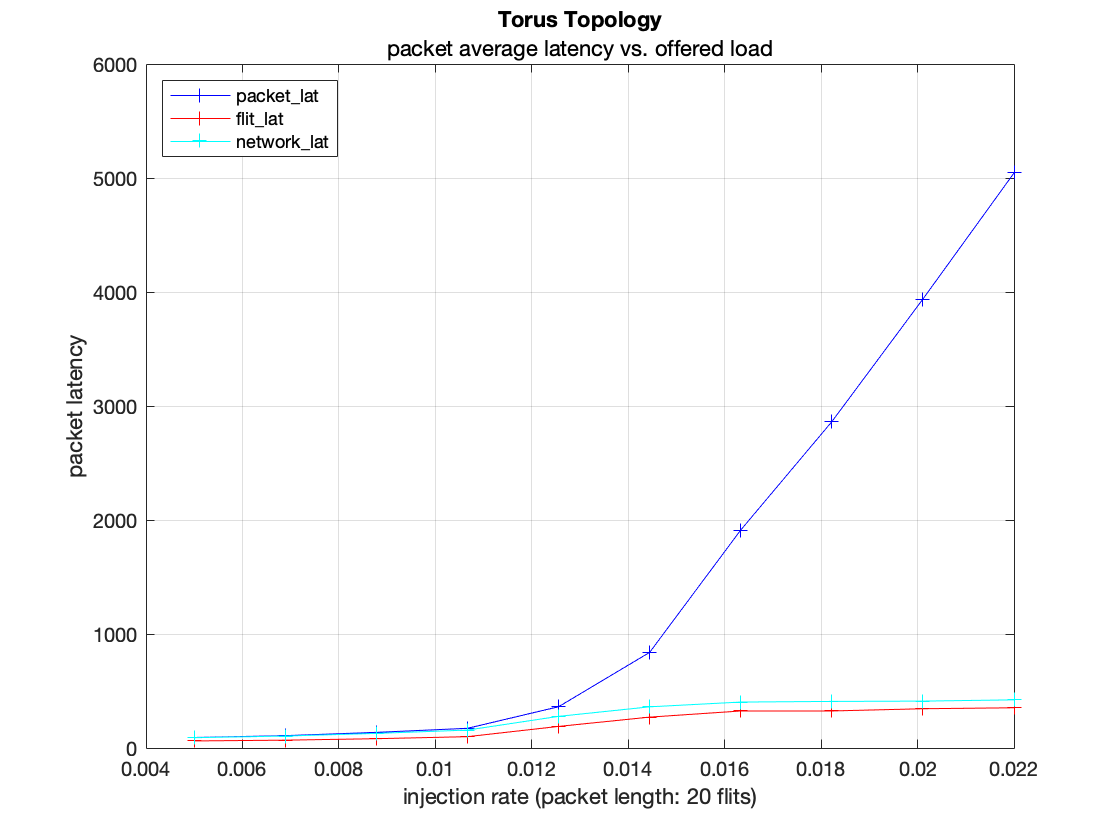
\includegraphics[width=0.45\textwidth]{Images/chap2/torus_tornado/torus_dor.png}
    %\caption{fig1}
    }
    \subfigure[valiant]{
    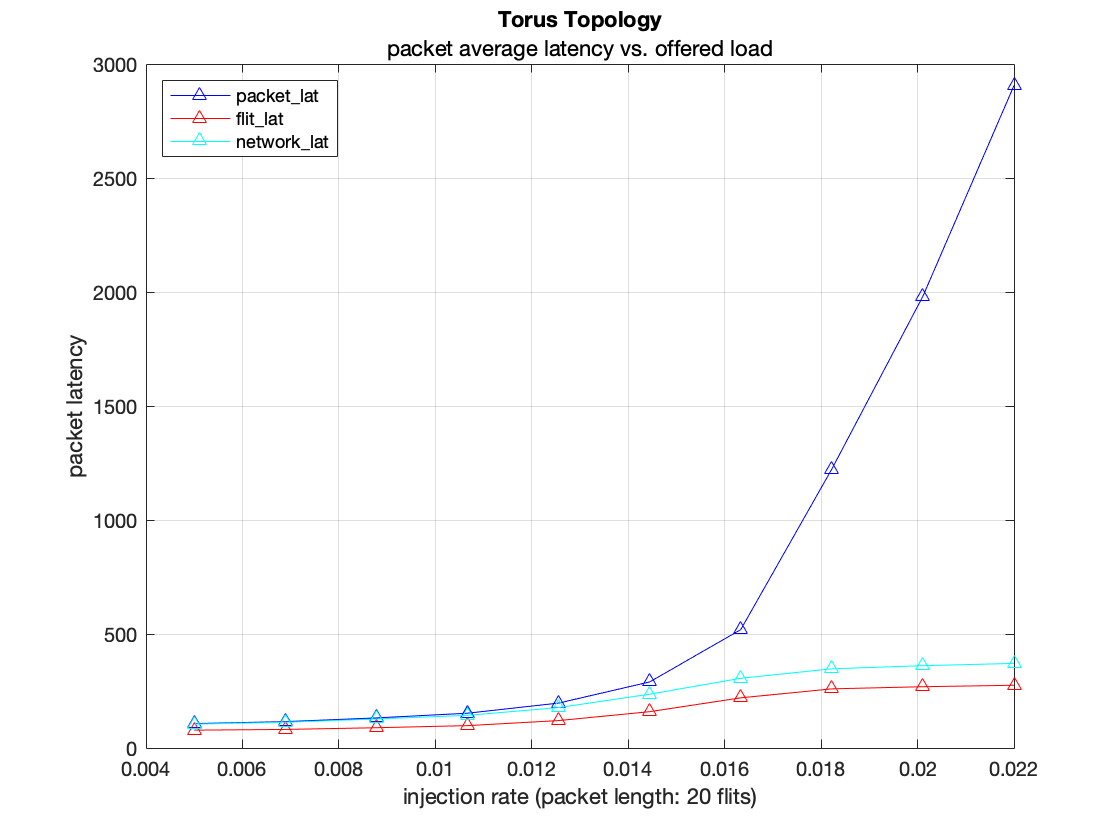
\includegraphics[width=0.45\textwidth]{Images/chap2/torus_tornado/torus_val.png}
    }
    \subfigure[minimal adaptive]{
    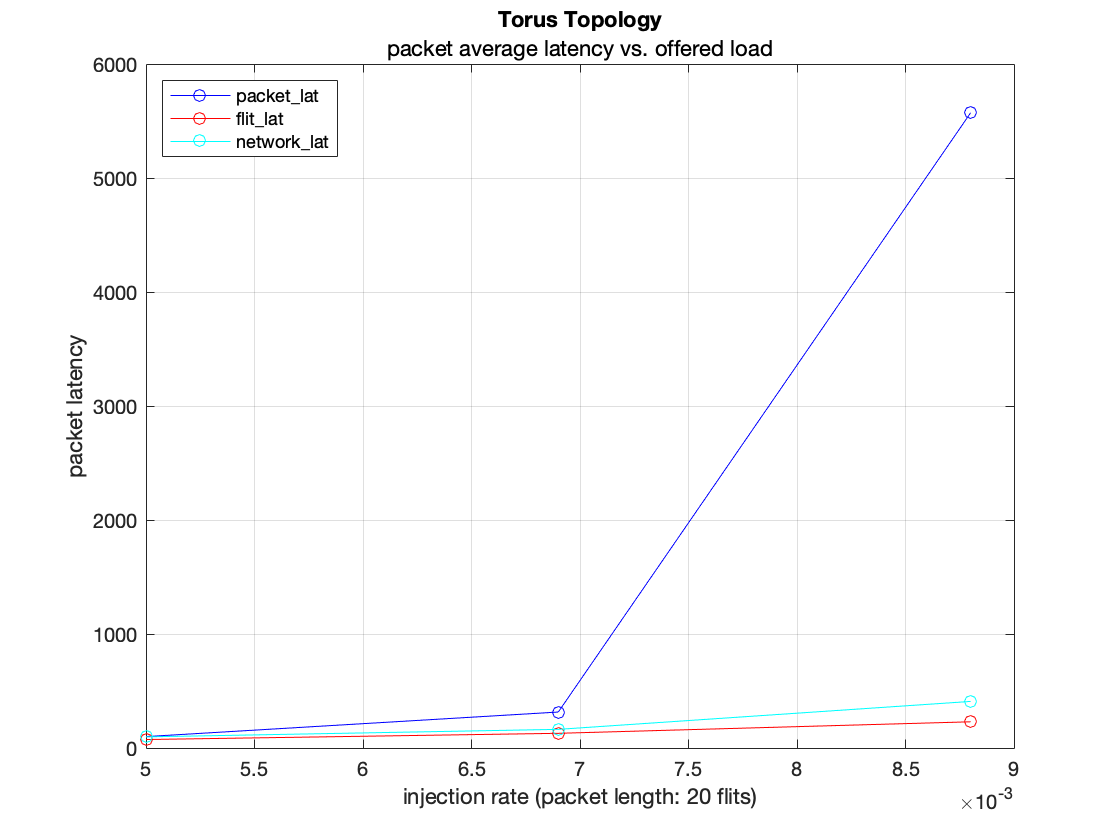
\includegraphics[width=0.45\textwidth]{Images/chap2/torus_tornado/torus_min.png}
    }
    \caption{Simulation results of Torus topology with uniform traffic}
    \label{fig:torus_tornado}
\end{figure}


\begin{figure}[H]
    \centering
    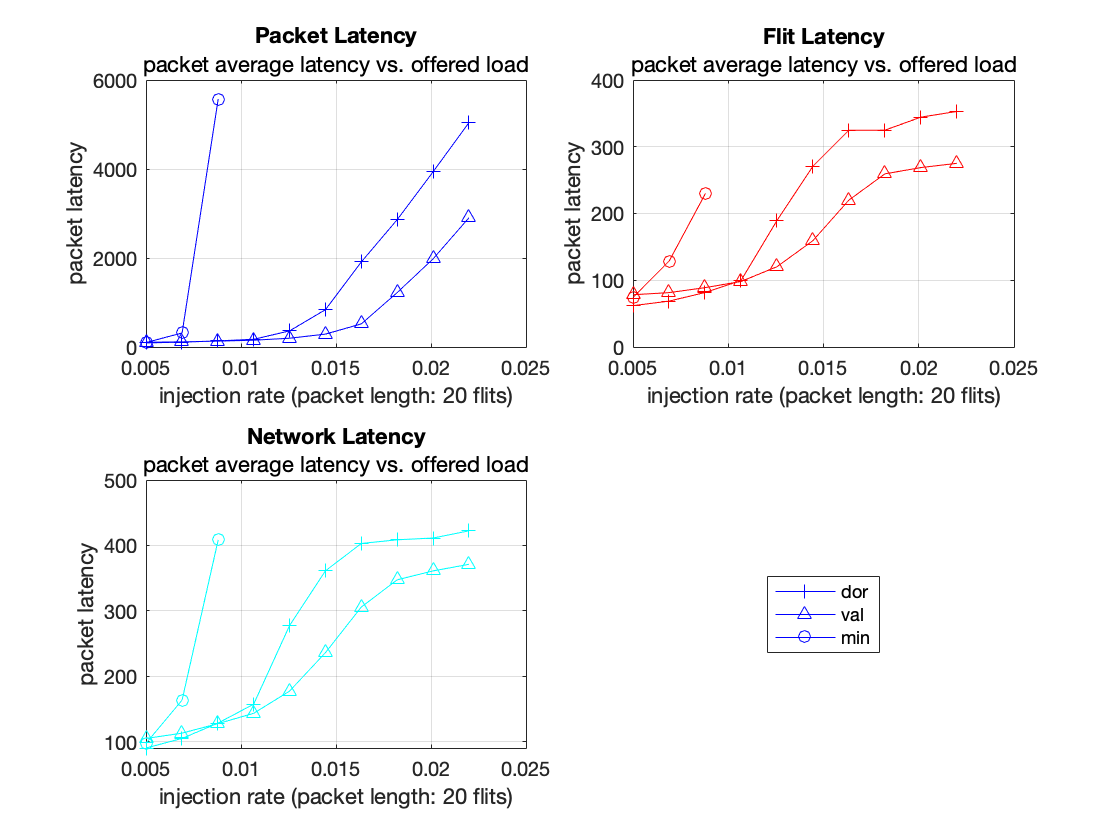
\includegraphics[width=0.9\textwidth]{Images/chap2/torus_tornado/torus_comparison.png}
    \caption{Latency comparison of 4 traffic patterns}
    \label{fig:com_torus_tornado}
\end{figure}



\subsection{Performance Comparison and Analysis}

The figure \ref{fig:com_tornado} compared the mesh and torus with different algorithms(DOR, VAL, MIN-ADAPT) separately. The DOR and MIN-ADAPT routing algorithms can support tornado traffic patterns in a mesh topology, and the corresponding performance of mesh topology is better than torus topology. However, the VAL routing algorithm performs better in torus topology under tornado traffic patterns. Overall, the VAL is suitable for Torus topology under tornado traffic patter. DOR is the suitable routing algorithm for mesh topology under tornado traffic patterns.

\begin{figure}[H]
    \centering
    \subfigure[dimension order]{
    \label{com_dor_tornado}
    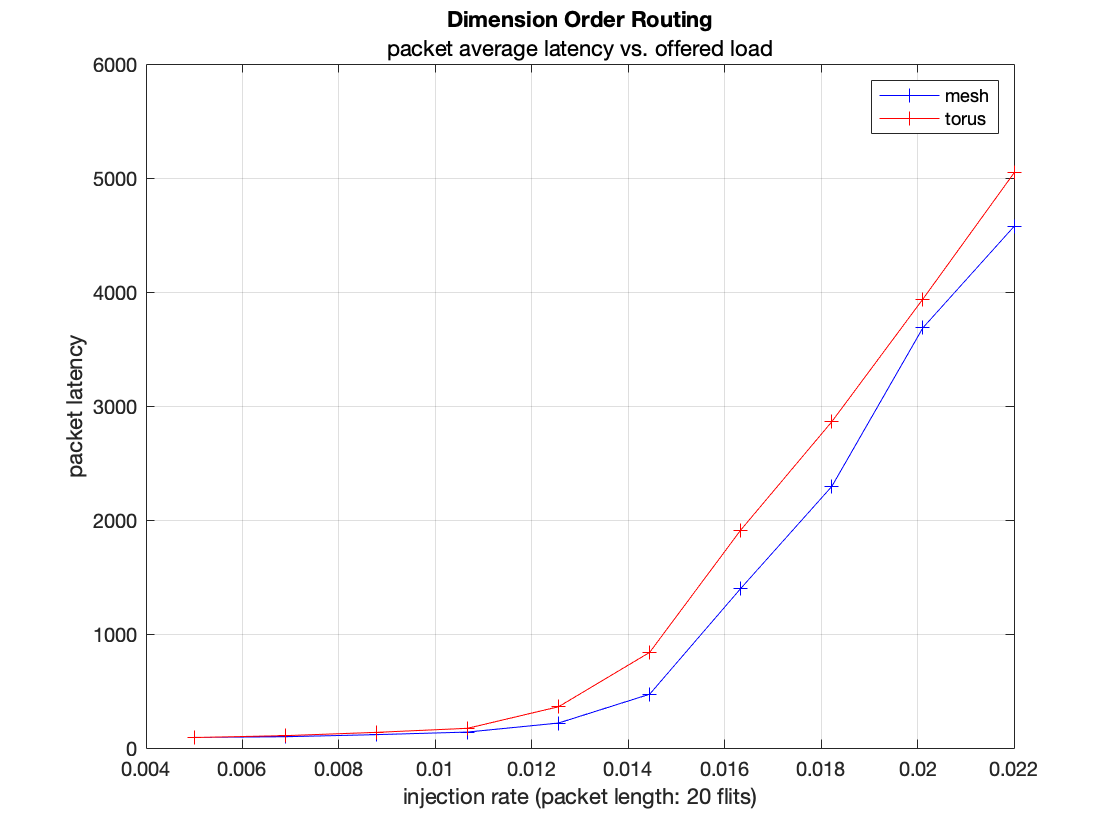
\includegraphics[width=0.45\textwidth]{Images/chap2/Comparison/Com_dor_tornado.png}
    %\caption{fig1}
    }
    \subfigure[valiant]{
    \label{com_val_tornado}
    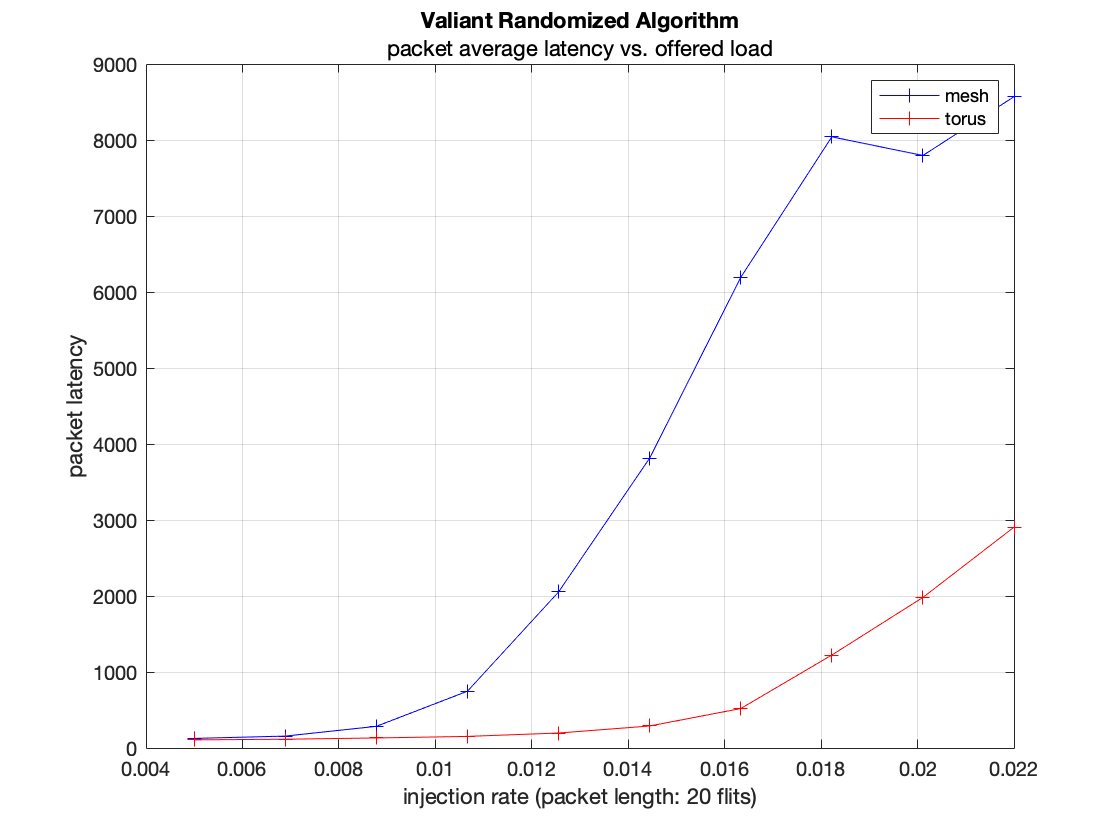
\includegraphics[width=0.45\textwidth]{Images/chap2/Comparison/Com_val_tornado.png}
    }
    \subfigure[minimal adaptive]{
    \label{com_min_tornado}
    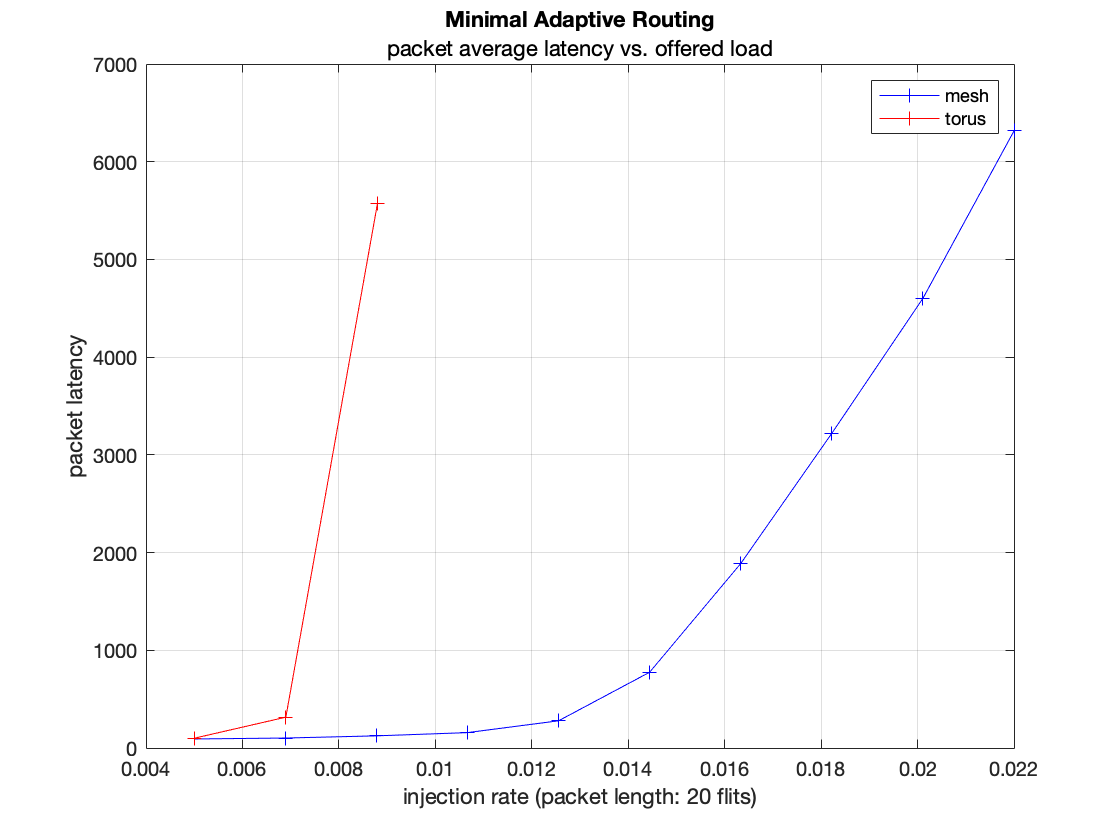
\includegraphics[width=0.45\textwidth]{Images/chap2/Comparison/Com_min_tornado.png}
    }
    \caption{Comparison under 'Tornado' traffic pattern}
    \label{fig:com_tornado}
\end{figure}


\section{Flow Control Comparison}
This additional experiment is executed under 'Mesh(ary8, dim2)' topology and 'uniform' traffic pattern.


\subsection{8 Virtual Channels, 8 buffer size per channel}
For the experiment results of this configuration, please refer to section \ref{sec:mesh_uniform}.

\subsection{4 Virtual Channels, 20 buffer size per channel}

\begin{longtable}[H]{llllll}
\centering
\label{tab:torus_tornado}
\textbf{topology} &
  \textbf{\begin{tabular}[c]{@{}l@{}}routing\\ \_algorithm\end{tabular}} &
  \textbf{\begin{tabular}[c]{@{}l@{}}injection\\ \_rate\end{tabular}} &
  \textbf{\begin{tabular}[c]{@{}l@{}}packet\\ \_size\end{tabular}} &
  \textbf{\begin{tabular}[c]{@{}l@{}}flow\\ \_control\end{tabular}} &
  \textbf{\begin{tabular}[c]{@{}l@{}}average\\ \_packet\\ \_delay\end{tabular}} \\ \hline
\endfirsthead %以上是最前的表头
\multicolumn{6}{c}{}\\

\textbf{topology} &
  \textbf{\begin{tabular}[c]{@{}l@{}}routing\\ \_algorithm\end{tabular}} &
  \textbf{\begin{tabular}[c]{@{}l@{}}injection\\ \_rate\end{tabular}} &
  \textbf{\begin{tabular}[c]{@{}l@{}}packet\\ \_size\end{tabular}} &
  \textbf{\begin{tabular}[c]{@{}l@{}}flow\\ \_control\end{tabular}} &
  \textbf{\begin{tabular}[c]{@{}l@{}}average\\ \_packet\\ \_delay\end{tabular}} \\ \hline
\endhead %以上是换页后的表头,如未换页,并不会显示
\hline
\multicolumn{6}{r}{Continue…}\\
\endfoot %以上是前页的表尾,如未换页,并不会显示。
\hline
\endlastfoot%以上选填最后也的表尾。一般不填
mesh(ary8,dim2) & dor        & 0.005  & 20 & 4\_20 & 70.976  \\
mesh(ary8,dim2) & dor        & 0.0069 & 20 & 4\_20 & 76.8099 \\
mesh(ary8,dim2) & dor        & 0.0088 & 20 & 4\_20 & 80.3712 \\
mesh(ary8,dim2) & dor        & 0.0107 & 20 & 4\_20 & 87.1603 \\
mesh(ary8,dim2) & dor        & 0.0126 & 20 & 4\_20 & 97.3517 \\
mesh(ary8,dim2) & dor        & 0.0144 & 20 & 4\_20 & 109.592 \\
mesh(ary8,dim2) & dor        & 0.0162 & 20 & 4\_20 & 127.506 \\
mesh(ary8,dim2) & dor        & 0.0182 & 20 & 4\_20 & 165.402 \\
mesh(ary8,dim2) & dor        & 0.0201 & 20 & 4\_20 & 304.805 \\
mesh(ary8,dim2) & dor        & 0.022  & 20 & 4\_20 & 1006.15 \\ \hline
mesh(ary8,dim2) & val        & 0.005  & 20 & 4\_20 & 127.754 \\
mesh(ary8,dim2) & val        & 0.0069 & 20 & 4\_20 & 155.127 \\
mesh(ary8,dim2) & val        & 0.0088 & 20 & 4\_20 & 249.517 \\
mesh(ary8,dim2) & val        & 0.0107 & 20 & 4\_20 & 1642.6  \\
mesh(ary8,dim2) & val        & 0.0126 & 20 & 4\_20 & 4275.11 \\
mesh(ary8,dim2) & val        & 0.0144 & 20 & 4\_20 &         \\
mesh(ary8,dim2) & val        & 0.0162 & 20 & 4\_20 &         \\
mesh(ary8,dim2) & val        & 0.0182 & 20 & 4\_20 &         \\
mesh(ary8,dim2) & val        & 0.0201 & 20 & 4\_20 &         \\
mesh(ary8,dim2) & val        & 0.022  & 20 & 4\_20 &         \\ \hline
mesh(ary8,dim2) & romm       & 0.005  & 20 & 4\_20 & 72.4624 \\
mesh(ary8,dim2) & romm       & 0.0069 & 20 & 4\_20 & 79.232  \\
mesh(ary8,dim2) & romm       & 0.0088 & 20 & 4\_20 & 83.2038 \\
mesh(ary8,dim2) & romm       & 0.0107 & 20 & 4\_20 & 95.5831 \\
mesh(ary8,dim2) & romm       & 0.0126 & 20 & 4\_20 & 112.182 \\
mesh(ary8,dim2) & romm       & 0.0144 & 20 & 4\_20 & 154.486 \\
mesh(ary8,dim2) & romm       & 0.0162 & 20 & 4\_20 & 994.973 \\
mesh(ary8,dim2) & romm       & 0.0182 & 20 & 4\_20 & 3016.01 \\
mesh(ary8,dim2) & romm       & 0.0201 & 20 & 4\_20 & 6296.15 \\
mesh(ary8,dim2) & romm       & 0.022  & 20 & 4\_20 &         \\ \hline
mesh(ary8,dim2) & min\_adapt & 0.005  & 20 & 4\_20 & 71.158  \\
mesh(ary8,dim2) & min\_adapt & 0.0069 & 20 & 4\_20 & 78.0626 \\
mesh(ary8,dim2) & min\_adapt & 0.0088 & 20 & 4\_20 & 83.0506 \\
mesh(ary8,dim2) & min\_adapt & 0.0107 & 20 & 4\_20 & 93.1438 \\
mesh(ary8,dim2) & min\_adapt & 0.0126 & 20 & 4\_20 & 111.268 \\
mesh(ary8,dim2) & min\_adapt & 0.0144 & 20 & 4\_20 & 132.44  \\
mesh(ary8,dim2) & min\_adapt & 0.0162 & 20 & 4\_20 & 194.157 \\
mesh(ary8,dim2) & min\_adapt & 0.0182 & 20 & 4\_20 & 281.173 \\
mesh(ary8,dim2) & min\_adapt & 0.0201 & 20 & 4\_20 & 641.147 \\
mesh(ary8,dim2) & min\_adapt & 0.022  & 20 & 4\_20 & 1467.9 
\end{longtable}

\begin{figure}[H]
    \centering
    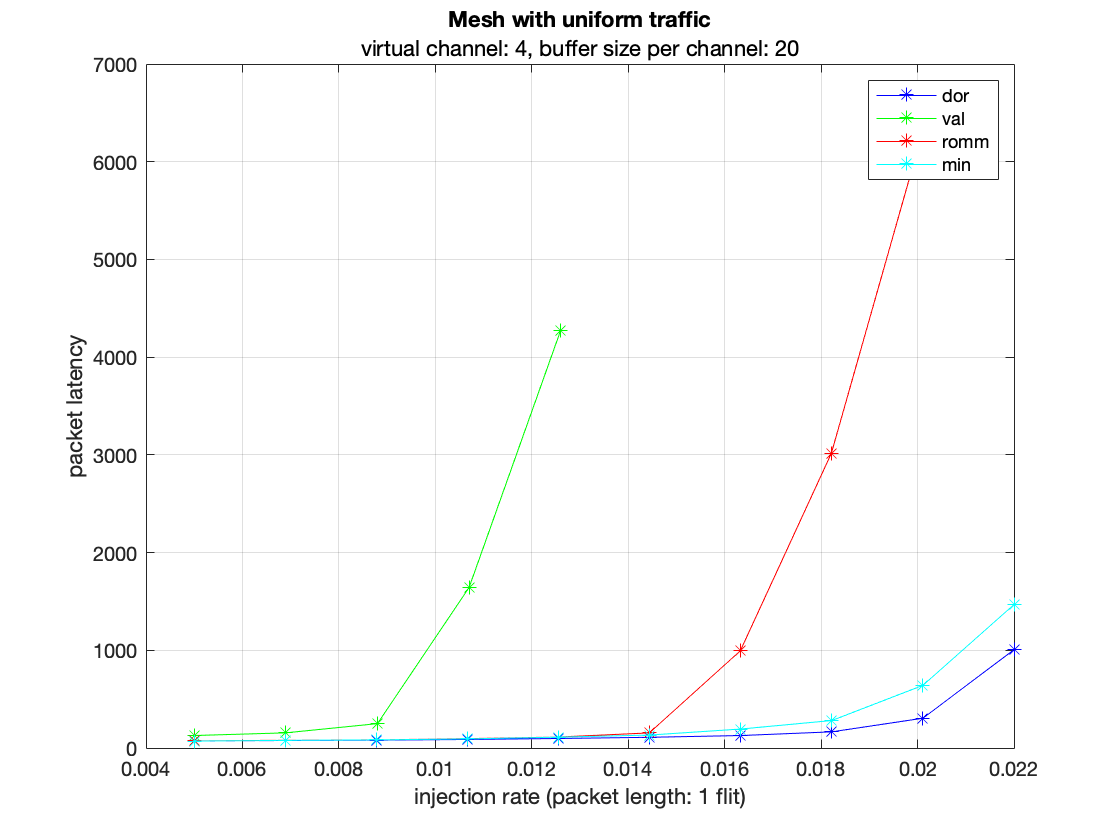
\includegraphics[width=0.9\textwidth]{Images/chap2/flow_control/fc4_20.png}
    \caption{Mesh topology with uniform traffic patter}
    \label{fig:mesh_fc420}
\end{figure}

In Fig. \ref{fig:mesh_fc820}, each curve represents a kind of routing algorithm under the same topology and traffic pattern; the performance of this configuration indicates that DOR is still the best routing algorithm for mesh topology, which is the same as we concluded in section \ref{sec:mesh_uniform_results}.


\subsection{8 Virtual Channels, 20 buffer size per channel}

% Please add the following required packages to your document preamble:
% \usepackage[table,xcdraw]{xcolor}
% If you use beamer only pass "xcolor=table" option, i.e. \documentclass[xcolor=table]{beamer}
\begin{longtable}[H]{llllll}
\centering
\label{tab:torus_tornado}
\textbf{topology} &
  \textbf{\begin{tabular}[c]{@{}l@{}}routing\\ \_algorithm\end{tabular}} &
  \textbf{\begin{tabular}[c]{@{}l@{}}injection\\ \_rate\end{tabular}} &
  \textbf{\begin{tabular}[c]{@{}l@{}}packet\\ \_size\end{tabular}} &
  \textbf{\begin{tabular}[c]{@{}l@{}}flow\\ \_control\end{tabular}} &
  \textbf{\begin{tabular}[c]{@{}l@{}}average\\ \_packet\\ \_delay\end{tabular}} \\ \hline
\endfirsthead %以上是最前的表头
\multicolumn{6}{c}{}\\

\textbf{topology} &
  \textbf{\begin{tabular}[c]{@{}l@{}}routing\\ \_algorithm\end{tabular}} &
  \textbf{\begin{tabular}[c]{@{}l@{}}injection\\ \_rate\end{tabular}} &
  \textbf{\begin{tabular}[c]{@{}l@{}}packet\\ \_size\end{tabular}} &
  \textbf{\begin{tabular}[c]{@{}l@{}}flow\\ \_control\end{tabular}} &
  \textbf{\begin{tabular}[c]{@{}l@{}}average\\ \_packet\\ \_delay\end{tabular}} \\ \hline
\endhead %以上是换页后的表头,如未换页,并不会显示
\hline
\multicolumn{6}{r}{Continue…}\\
\endfoot %以上是前页的表尾,如未换页,并不会显示。
\hline
\endlastfoot%以上选填最后也的表尾。一般不填
mesh(ary8,dim2) & dor        & 0.005  & 20 & 8\_20 & 71.1348 \\
mesh(ary8,dim2) & dor        & 0.0069 & 20 & 8\_20 & 76.9622 \\
mesh(ary8,dim2) & dor        & 0.0088 & 20 & 8\_20 & 80.4911 \\
mesh(ary8,dim2) & dor        & 0.0107 & 20 & 8\_20 & 87.7844 \\
mesh(ary8,dim2) & dor        & 0.0126 & 20 & 8\_20 & 98.2077 \\
mesh(ary8,dim2) & dor        & 0.0144 & 20 & 8\_20 & 112.963 \\
mesh(ary8,dim2) & dor        & 0.0162 & 20 & 8\_20 & 135.599 \\
mesh(ary8,dim2) & dor        & 0.0182 & 20 & 8\_20 & 169.159 \\
mesh(ary8,dim2) & dor        & 0.0201 & 20 & 8\_20 & 247.456 \\
mesh(ary8,dim2) & dor        & 0.022  & 20 & 8\_20 & 542.698 \\ \hline
mesh(ary8,dim2) & val        & 0.005  & 20 & 8\_20 & 128.261 \\
mesh(ary8,dim2) & val        & 0.0069 & 20 & 8\_20 & 155.178 \\
mesh(ary8,dim2) & val        & 0.0088 & 20 & 8\_20 & 238.409 \\
mesh(ary8,dim2) & val        & 0.0107 & 20 & 8\_20 & 738.991 \\
mesh(ary8,dim2) & val        & 0.0126 & 20 & 8\_20 & 3624.72 \\
mesh(ary8,dim2) & val        & 0.0144 & 20 & 8\_20 & 4687.82 \\
mesh(ary8,dim2) & val        & 0.0162 & 20 & 8\_20 &         \\
mesh(ary8,dim2) & val        & 0.0182 & 20 & 8\_20 &         \\
mesh(ary8,dim2) & val        & 0.0201 & 20 & 8\_20 &         \\
mesh(ary8,dim2) & val        & 0.022  & 20 & 8\_20 &         \\ \hline
mesh(ary8,dim2) & romm       & 0.005  & 20 & 8\_20 & 72.8313 \\
mesh(ary8,dim2) & romm       & 0.0069 & 20 & 8\_20 & 80.3477 \\
mesh(ary8,dim2) & romm       & 0.0088 & 20 & 8\_20 & 84.3721 \\
mesh(ary8,dim2) & romm       & 0.0107 & 20 & 8\_20 & 95.5874 \\
mesh(ary8,dim2) & romm       & 0.0126 & 20 & 8\_20 & 112.338 \\
mesh(ary8,dim2) & romm       & 0.0144 & 20 & 8\_20 & 135.455 \\
mesh(ary8,dim2) & romm       & 0.0162 & 20 & 8\_20 & 203.494 \\
mesh(ary8,dim2) & romm       & 0.0182 & 20 & 8\_20 & 874.43  \\
mesh(ary8,dim2) & romm       & 0.0201 & 20 & 8\_20 &         \\
mesh(ary8,dim2) & romm       & 0.022  & 20 & 8\_20 &         \\ \hline
mesh(ary8,dim2) & min\_adapt & 0.005  & 20 & 8\_20 & 71.5045 \\
mesh(ary8,dim2) & min\_adapt & 0.0069 & 20 & 8\_20 & 78.1588 \\
mesh(ary8,dim2) & min\_adapt & 0.0088 & 20 & 8\_20 & 82.9398 \\
mesh(ary8,dim2) & min\_adapt & 0.0107 & 20 & 8\_20 & 92.3613 \\
mesh(ary8,dim2) & min\_adapt & 0.0126 & 20 & 8\_20 & 106.342 \\
mesh(ary8,dim2) & min\_adapt & 0.0144 & 20 & 8\_20 & 138.05  \\
mesh(ary8,dim2) & min\_adapt & 0.0162 & 20 & 8\_20 & 188.865 \\
mesh(ary8,dim2) & min\_adapt & 0.0182 & 20 & 8\_20 & 270.352 \\
mesh(ary8,dim2) & min\_adapt & 0.0201 & 20 & 8\_20 & 391.475 \\
mesh(ary8,dim2) & min\_adapt & 0.022  & 20 & 8\_20 & 766.477
\end{longtable}

\begin{figure}[H]
    \centering
    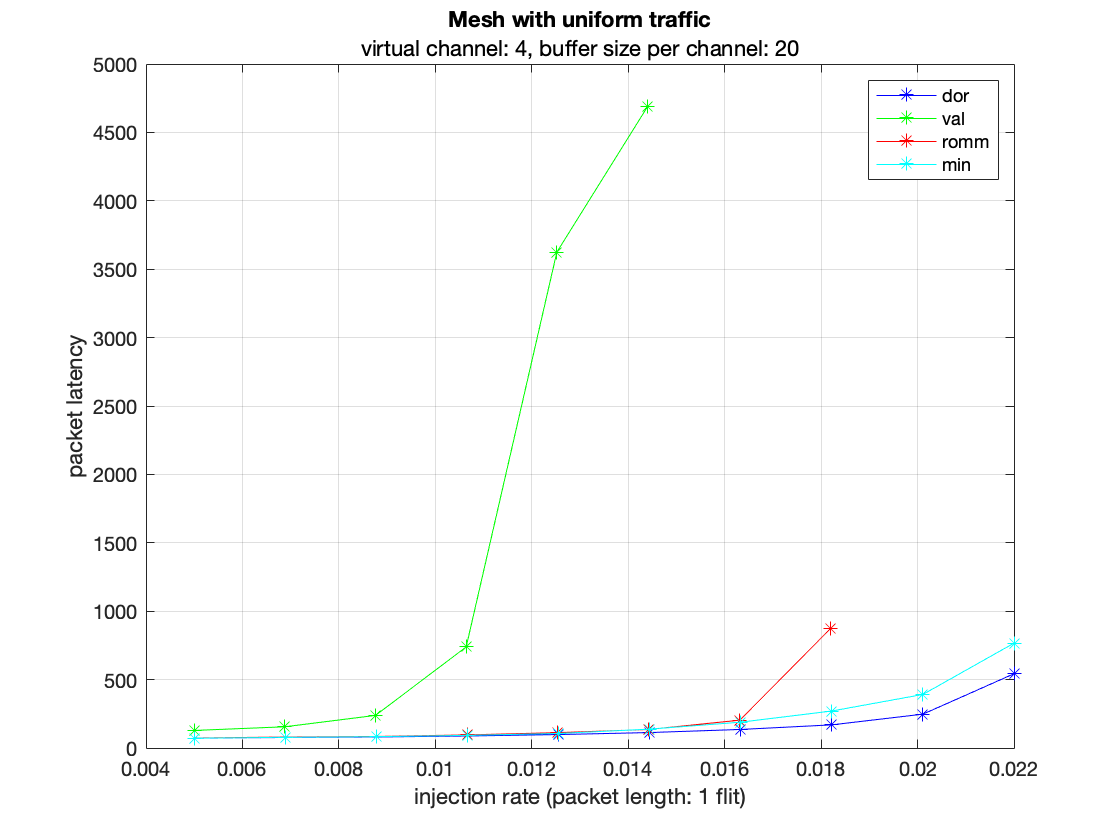
\includegraphics[width=0.9\textwidth]{Images/chap2/flow_control/fc8_20.png}
    \caption{Mesh topology with uniform traffic patter}
    \label{fig:mesh_fc820}
\end{figure}

In Fig. \ref{fig:mesh_fc820}, each curve represent a kind of routing algorithm under the same topology and traffic pattern, the performance of this configuration indicates that DOR is still the best routing algorithm for mesh topology which is the same as we concluded in section \ref{sec:mesh_uniform_results}.

\subsubsection{Comprehensive Comparison}
According to Fig. \ref{fig:mesh_fc420} and Fig. \ref{fig:mesh_fc820}, we can find that for the same topology(mesh) and the same traffic pattern(uniform), the performance with more virtual channels will have lower latency. However, the latency does not always decrease with the increment of the virtual channel number. 


\chapter{Assignment 2} \label{chap-3}
\textbf{Implement your own network topologies and evaluate the performance}\\
The detailed description of this assignment can be found here: \href{https://seis.bristol.ac.uk/~sy13201/DCN/Lab\%20Note.html}{Lab Note for Data Center Networking} or go to the next url: \url{https://seis.bristol.ac.uk/~sy13201/DCN/Lab\%20Note.html}


\section{Use booksim to evaluate the performance of a network topology designed in the guidance}



\subsection{Define performance metric for the evaluation}
\label{sec:3.1.1}
We will test the \textbf{latency} with different combinations of the parameters in the configuration file. (e.g., packet size, virtual channel)
    
\subsection{Results and discussion for the evaluation}

% Please add the following required packages to your document preamble:
% \usepackage[table,xcdraw]{xcolor}
% If you use beamer only pass "xcolor=table" option, i.e. \documentclass[xcolor=table]{beamer}
\begin{longtable}[H]{llllll}
\centering
\label{tab:torus_tornado}
\textbf{topology} &
  \cellcolor[HTML]{00B0F0}\textbf{\begin{tabular}[c]{@{}l@{}}injection\\ \_rate\end{tabular}} &
  \textbf{Traffic} &
  \cellcolor[HTML]{00B0F0}\textbf{\begin{tabular}[c]{@{}l@{}}packet\\ \_size\end{tabular}} &
  \cellcolor[HTML]{00B0F0}\textbf{\begin{tabular}[c]{@{}l@{}}flow\\ \_control\end{tabular}} &
  \textbf{\begin{tabular}[c]{@{}l@{}}average\\ \_packet\\ \_delay\end{tabular}} \\ \hline
\endfirsthead %以上是最前的表头
\multicolumn{6}{c}{}\\

\textbf{topology} &
  \cellcolor[HTML]{00B0F0}\textbf{\begin{tabular}[c]{@{}l@{}}injection\\ \_rate\end{tabular}} &
  \textbf{Traffic} &
  \cellcolor[HTML]{00B0F0}\textbf{\begin{tabular}[c]{@{}l@{}}packet\\ \_size\end{tabular}} &
  \cellcolor[HTML]{00B0F0}\textbf{\begin{tabular}[c]{@{}l@{}}flow\\ \_control\end{tabular}} &
  \textbf{\begin{tabular}[c]{@{}l@{}}average\\ \_packet\\ \_delay\end{tabular}} \\ \hline
\endhead %以上是换页后的表头,如未换页,并不会显示
\hline
\multicolumn{6}{r}{Continue…}\\
\endfoot %以上是前页的表尾,如未换页,并不会显示。
\hline
\endlastfoot%以上选填最后也的表尾。一般不填


testnet(r4,e3) & 0.55 & uniform & 1 & default & 9.00424 \\
testnet(r4,e3) & 0.6  & uniform & 1 & default & 9.55989 \\
testnet(r4,e3) & 0.65 & uniform & 1 & default & 11.4555 \\
testnet(r4,e3) & 0.7  & uniform & 1 & default & 15.3622 \\
testnet(r4,e3) & 0.75 & uniform & 1 & default & 36.1957 \\
testnet(r4,e3) & 0.8  & uniform & 1 & default & 50.0457 \\
testnet(r4,e3) & 0.85 & uniform & 1 & default & 87.4587 \\
testnet(r4,e3) & 0.9  & uniform & 1 & default & 114.525 \\
testnet(r4,e3) & 0.95 & uniform & 1 & default & 165.763 \\
testnet(r4,e3) & 1    & uniform & 1 & default & 209.438 \\ \hline
testnet(r4,e3) & 0.55 & uniform & 5 & default & 1035.9  \\
testnet(r4,e3) & 0.6  & uniform & 5 & default & 1178.85 \\
testnet(r4,e3) & 0.65 & uniform & 5 & default & 1303.66 \\
testnet(r4,e3) & 0.7  & uniform & 5 & default & 1452.35 \\
testnet(r4,e3) & 0.75 & uniform & 5 & default & 1569.47 \\
testnet(r4,e3) & 0.8  & uniform & 5 & default & 1714.97 \\
testnet(r4,e3) & 0.85 & uniform & 5 & default & 1842.04 \\
testnet(r4,e3) & 0.9  & uniform & 5 & default & 1966.17 \\
testnet(r4,e3) & 0.95 & uniform & 5 & default & 2091.34 \\
testnet(r4,e3) & 1    & uniform & 5 & default & 2221.98 \\ \hline
testnet(r4,e3) & 0.55 & uniform & 1 & 6       & 8.89958 \\
testnet(r4,e3) & 0.6  & uniform & 1 & 6       & 9.46639 \\
testnet(r4,e3) & 0.65 & uniform & 1 & 6       & 10.9079 \\
testnet(r4,e3) & 0.7  & uniform & 1 & 6       & 14.5966 \\
testnet(r4,e3) & 0.75 & uniform & 1 & 6       & 33.1129 \\
testnet(r4,e3) & 0.8  & uniform & 1 & 6       & 48.5042 \\
testnet(r4,e3) & 0.85 & uniform & 1 & 6       & 85.7041 \\
testnet(r4,e3) & 0.9  & uniform & 1 & 6       & 129.583 \\
testnet(r4,e3) & 0.95 & uniform & 1 & 6       & 160.373 \\
testnet(r4,e3) & 1    & uniform & 1 & 6       & 210.397 \\ \hline
testnet(r4,e3) & 0.55 & uniform & 1 & 6       & 1037.71 \\
testnet(r4,e3) & 0.6  & uniform & 1 & 6       & 1178.58 \\
testnet(r4,e3) & 0.65 & uniform & 1 & 6       & 1303.54 \\
testnet(r4,e3) & 0.7  & uniform & 1 & 6       & 1452.23 \\
testnet(r4,e3) & 0.75 & uniform & 1 & 6       & 1571.02 \\
testnet(r4,e3) & 0.8  & uniform & 1 & 6       & 1714.49 \\
testnet(r4,e3) & 0.85 & uniform & 1 & 6       & 1844.23 \\
testnet(r4,e3) & 0.9  & uniform & 1 & 6       & 1968.37 \\
testnet(r4,e3) & 0.95 & uniform & 1 & 6       & 2093.63 \\
testnet(r4,e3) & 1    & uniform & 1 & 6       & 2224.28 
\end{longtable}

\begin{figure}[H]
    \centering
    \subfigure[p1]{
    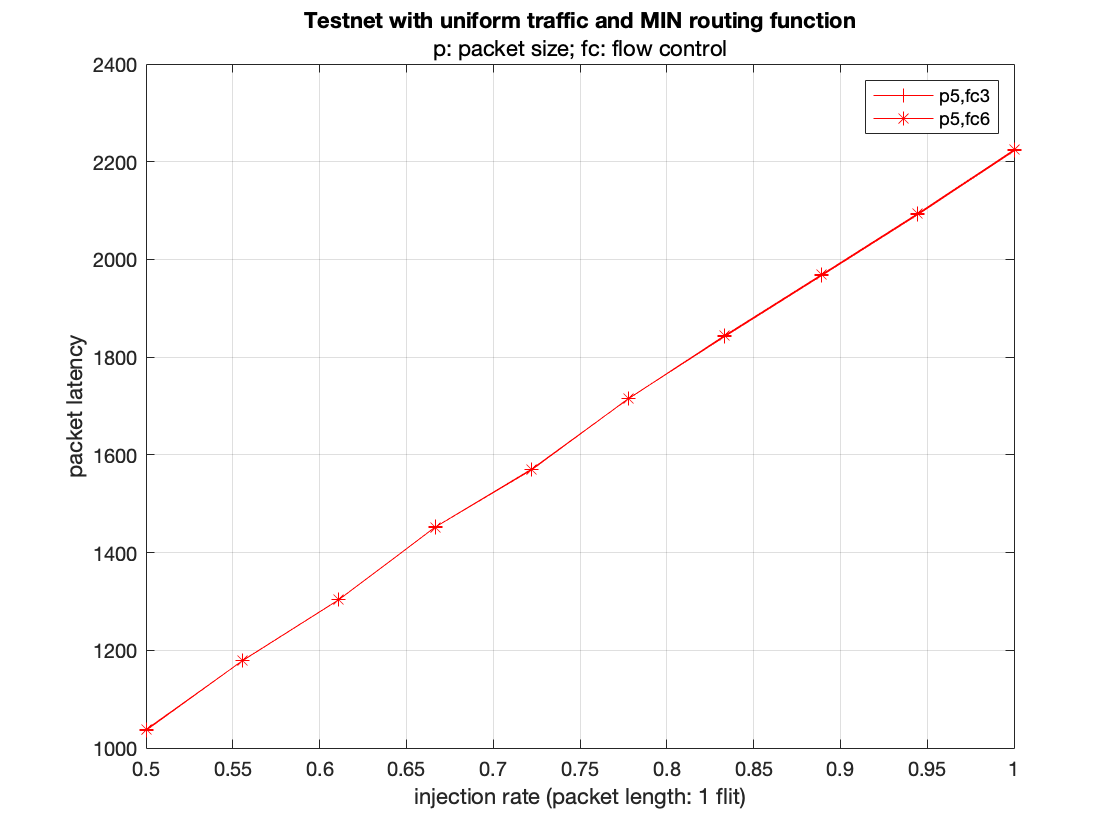
\includegraphics[width=0.45\textwidth]{Images/chap3/2_1_1.png}
    }
    \subfigure[p5]{
    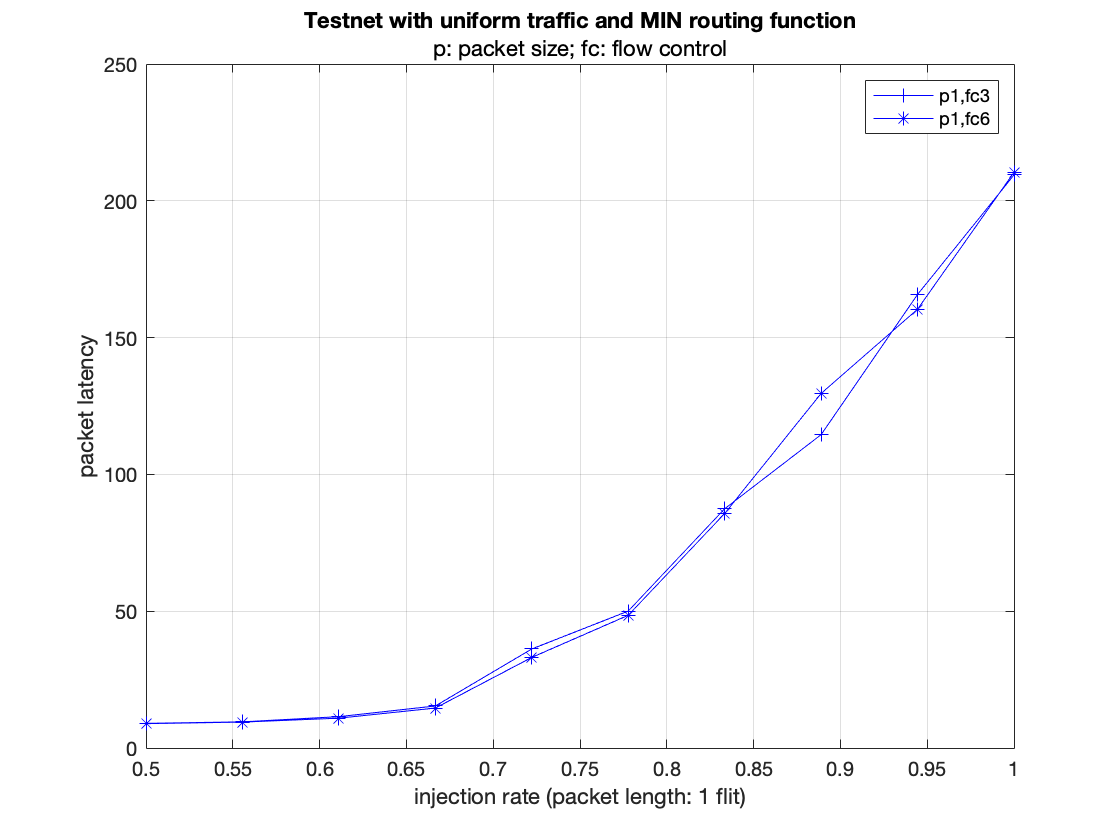
\includegraphics[width=0.45\textwidth]{Images/chap3/2_1_2.png}
    }
    \caption{Simulation results testnet}
    \label{fig:testnet_1}
\end{figure}

From Fig. \ref{fig:testnet_1}, we can find that the latency is always increasing with the increments of the injection rates. Under packet size of 1, the performances with virtual channels of 3 and 6 are almost the same. Under packet size of 5, the performances with virtual channels of 3 and 6 are slightly different.


\section{Build your own network}

\subsection{Build the network}
Build a network with the name as DesignNet. It includes 8 routers and 32 nodes. Between routers, the links drawn in the figures are bidirectional links. Here we assume a fully connected network is setup between all routers. Some links between routers are omitted for simplicity. Create the network and evaluate the performance.

% Please add the following required packages to your document preamble:
% \usepackage[table,xcdraw]{xcolor}
% If you use beamer only pass "xcolor=table" option, i.e. \documentclass[xcolor=table]{beamer}
\begin{longtable}[H]{llllll}
\centering
\label{tab:torus_tornado}
\textbf{topology} &
  \cellcolor[HTML]{00B0F0}\textbf{\begin{tabular}[c]{@{}l@{}}injection\\ \_rate\end{tabular}} &
  \textbf{Traffic} &
  \cellcolor[HTML]{00B0F0}\textbf{\begin{tabular}[c]{@{}l@{}}packet\\ \_size\end{tabular}} &
  \cellcolor[HTML]{00B0F0}\textbf{\begin{tabular}[c]{@{}l@{}}flow\\ \_control\end{tabular}} &
  \textbf{\begin{tabular}[c]{@{}l@{}}average\\ \_packet\\ \_delay\end{tabular}} \\ \hline
\endfirsthead %以上是最前的表头
\multicolumn{6}{c}{}\\

\textbf{topology} &
  \cellcolor[HTML]{00B0F0}\textbf{\begin{tabular}[c]{@{}l@{}}injection\\ \_rate\end{tabular}} &
  \textbf{Traffic} &
  \cellcolor[HTML]{00B0F0}\textbf{\begin{tabular}[c]{@{}l@{}}packet\\ \_size\end{tabular}} &
  \cellcolor[HTML]{00B0F0}\textbf{\begin{tabular}[c]{@{}l@{}}flow\\ \_control\end{tabular}} &
  \textbf{\begin{tabular}[c]{@{}l@{}}average\\ \_packet\\ \_delay\end{tabular}} \\ \hline
\endhead %以上是换页后的表头,如未换页,并不会显示
\hline
\multicolumn{6}{r}{Continue…}\\
\endfoot %以上是前页的表尾,如未换页,并不会显示。
\hline
\endlastfoot%以上选填最后也的表尾。一般不填

testnet(r4,e3) & 0.55 & uniform & 1 & default & 9.34287 \\
testnet(r4,e3) & 0.6  & uniform & 1 & default & 10.0335 \\
testnet(r4,e3) & 0.65 & uniform & 1 & default & 11.4095 \\
testnet(r4,e3) & 0.7  & uniform & 1 & default & 14.6115 \\
testnet(r4,e3) & 0.75 & uniform & 1 & default & 23.1209 \\
testnet(r4,e3) & 0.8  & uniform & 1 & default & 45.322  \\
testnet(r4,e3) & 0.85 & uniform & 1 & default & 84.0369 \\
testnet(r4,e3) & 0.9  & uniform & 1 & default & 119.761 \\
testnet(r4,e3) & 0.95 & uniform & 1 & default & 158.2   \\
testnet(r4,e3) & 1    & uniform & 1 & default & 192.858 \\
testnet(r4,e3) & 0.55 & uniform & 5 & default & 1048.03 \\
testnet(r4,e3) & 0.6  & uniform & 5 & default & 1181.38 \\
testnet(r4,e3) & 0.65 & uniform & 5 & default & 1310.65 \\
testnet(r4,e3) & 0.7  & uniform & 5 & default & 1444.5  \\
testnet(r4,e3) & 0.75 & uniform & 5 & default & 1574.2  \\
testnet(r4,e3) & 0.8  & uniform & 5 & default & 1707.99 \\
testnet(r4,e3) & 0.85 & uniform & 5 & default & 1839.84 \\
testnet(r4,e3) & 0.9  & uniform & 5 & default & 1965.54 \\
testnet(r4,e3) & 0.95 & uniform & 5 & default & 2088.24 \\
testnet(r4,e3) & 1    & uniform & 5 & default & 2218.58 \\
testnet(r4,e3) & 0.55 & uniform & 1 & 6       & 9.27776 \\
testnet(r4,e3) & 0.6  & uniform & 1 & 6       & 9.91647 \\
testnet(r4,e3) & 0.65 & uniform & 1 & 6       & 11.266  \\
testnet(r4,e3) & 0.7  & uniform & 1 & 6       & 14.5709 \\
testnet(r4,e3) & 0.75 & uniform & 1 & 6       & 22.3257 \\
testnet(r4,e3) & 0.8  & uniform & 1 & 6       & 48.0027 \\
testnet(r4,e3) & 0.85 & uniform & 1 & 6       & 89.5332 \\
testnet(r4,e3) & 0.9  & uniform & 1 & 6       & 117.538 \\
testnet(r4,e3) & 0.95 & uniform & 1 & 6       & 154.02  \\
testnet(r4,e3) & 1    & uniform & 1 & 6       & 196.502 \\
testnet(r4,e3) & 0.55 & uniform & 1 & 6       & 1048.27 \\
testnet(r4,e3) & 0.6  & uniform & 1 & 6       & 1180.26 \\
testnet(r4,e3) & 0.65 & uniform & 1 & 6       & 1309.58 \\
testnet(r4,e3) & 0.7  & uniform & 1 & 6       & 1442.91 \\
testnet(r4,e3) & 0.75 & uniform & 1 & 6       & 1576.07 \\
testnet(r4,e3) & 0.8  & uniform & 1 & 6       & 1707.35 \\
testnet(r4,e3) & 0.85 & uniform & 1 & 6       & 1840.15 \\
testnet(r4,e3) & 0.9  & uniform & 1 & 6       & 1966.2  \\
testnet(r4,e3) & 0.95 & uniform & 1 & 6       & 2088.38 \\
testnet(r4,e3) & 1    & uniform & 1 & 6       & 2218.73 \\
\end{longtable}

\begin{figure}[H]
    \centering
    \subfigure[p1]{
    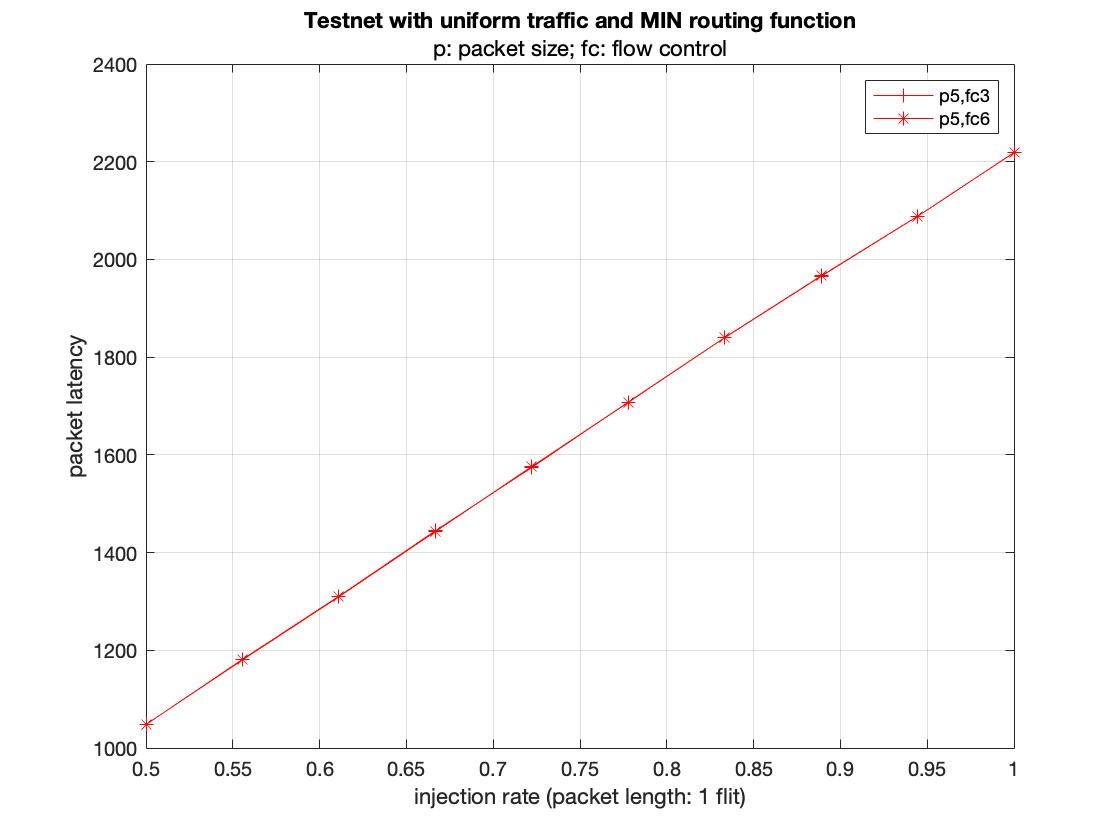
\includegraphics[width=0.45\textwidth]{Images/chap3/2_2_1.png}
    }
    \subfigure[p5]{
    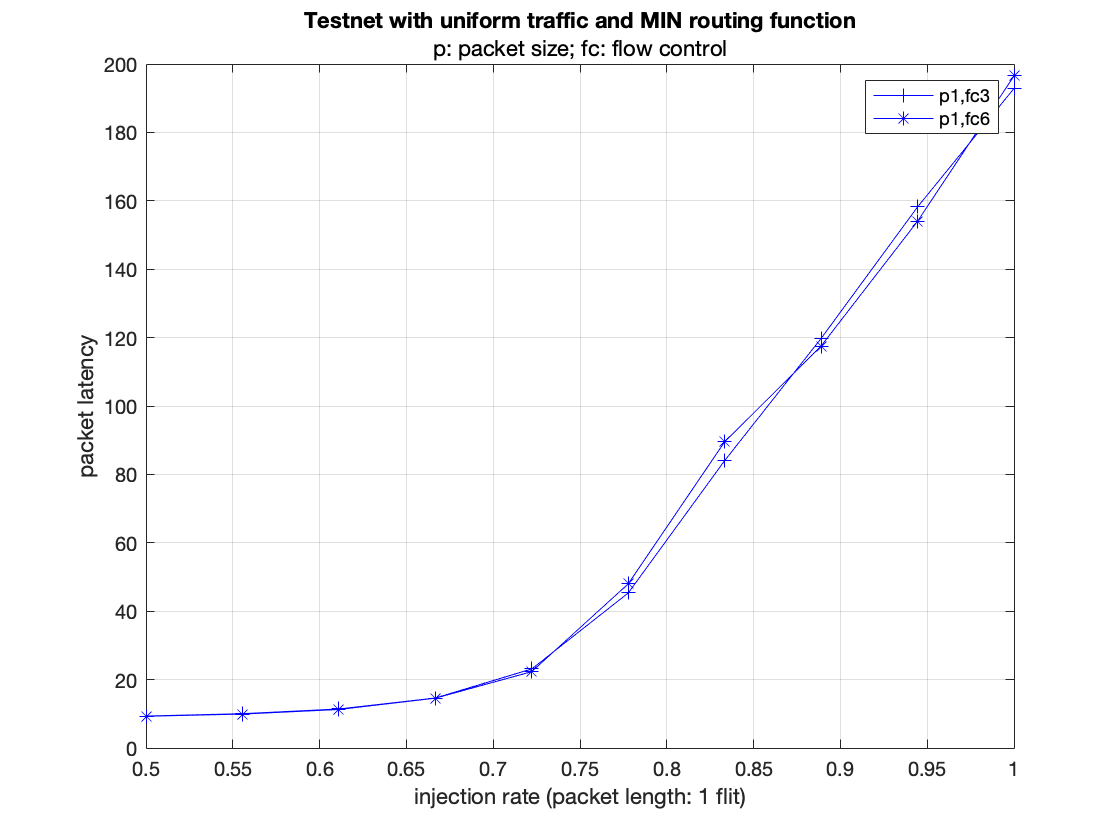
\includegraphics[width=0.45\textwidth]{Images/chap3/2_2_2.png}
    }
    \caption{Simulation results testnet}
    \label{fig:testnet_2}
\end{figure}

From Fig. \ref{fig:testnet_2}, we can find that the latency is always increasing with the increments of the injection rates. Under packet size of 1, the performances with virtual channels of 3 and 6 are almost the same. Under packet size of 5, the performances with virtual channels of 3 and 6 are slightly different.

\subsection{Evaluation}
Evaluate the performance based on the metrics defined in \ref{sec:3.1.1}.

From all the simulation results above, it is impossible to determine which routing algorithm is the best and under what kind of flow control we can get the best performance. Since the performance of a network system not only depends on the topology itself, the traffic patterns, packet size, injection rates, and flow control will all impact the performance of such a network system.

 
%\input{MainText/chapter4} 
%\input{MainText/chapter5} 

%----------------------------------------------------------------------------------------
%	BIBLIOGRAPHY
%----------------------------------------------------------------------------------------

% \addtocontents{toc}{\vspace{2em}} % Add a gap in the Contents, for aesthetics
% \unnumberedchapter{Reference} % Title of the unnumbered chapter
% \bibliography{Preamble/Thesis_bibliography} % The references information are stored in the file named "Thesis_bibliography.bib"

%----------------------------------------------------------------------------------------
%	APPENDICES
%----------------------------------------------------------------------------------------

\addtocontents{toc}{\vspace{2em}} % Add a gap in the Contents, for aesthetics
\appendix % Starts of appendices

\numberedchapter
\chapter{Simulation Package}
The attached booksim.zip file contains all the source code of the simulaiton platform and some Python scripts for efficiency. The place of the newly added files mostly in path booksim/src/project.
The Python scripts for modifying and executing simulations are under the path booksim/src, they are named Datacenter\_00x.py (x is in range from 1 to 4). The simulation results will be stored in the path booksim/src/project/results. Before running the script, please read the codes and create corresponding folder under the path booksim/src/project/results.

For the data extraction part, under the simulation results folder(e.g., booksim/src/project/results/testnet\_dir\_p1), there will be a python script named data\_collection.py. 
Running this file, you will get a newly created file under this path, all the data we needed for reports is extracted and stored in this file(e.g., Testnetconfig\_res).
%\input{MainText/appendixB}
%\input{MainText/appendixC}

\end{document}  